%================================================================
% SLO: definiraj strukturo dokumenta
% ENG: define file structure
%================================================================
\documentclass[a4paper, 12pt]{book}
 

%================================================================
% SLO: Odkomentiraj "\SLOtrue " za izbiro slovenskega jezika
% ENG: Uncomment "\SLOfalse" to chose English languagge
%================================================================
\newif\ifSLO
\newif\ifTRACKEXIST
\newif\ifTRACKCS
\newif\ifPROGRAMMM
\newif\ifPROGRAMEMAI

% ---------------------------------------------------------------------------------------
% IMPORTANT: Adjust the thesis language, your study program and track within this block
% ---------------------------------------------------------------------------------------
% ** switch language ** %
\SLOtrue % Enables Slovenian language
%\SLOfalse  % Enables English language

% ** Switch programs: ** %

% ** Uncomment if Program: Computer Science, Track: Computer Science **%
\TRACKCStrue
\TRACKEXISTtrue

% ** Uncomment if Program: Computer Science, Track: Data Science **%
%\TRACKCSfalse
%\TRACKEXISTtrue

% ** Uncomment if Program: Multimedia **%
%\PROGRAMMMtrue 
%\TRACKEXISTfalse 

% ** Uncomment if Program: EMAI **%
%\PROGRAMEMAItrue
%\SLOfalse 

% -------------------------------------------------------------------------------------------
% End of language, program and track adjustment
% -------------------------------------------------------------------------------------------


%================================================================
% SLO: vključi oblikovanje in pakete
% ENG: include design and packages
%================================================================
\input{style/thesis_style}

%----------------------------------------------------------------
% |||||||||||||||||||||| USTREZNO POPRAVI |||||||||||||||||||||||
% |||||||||||||||||||||| EDIT ACCORDINGLY |||||||||||||||||||||||
%----------------------------------------------------------------
\newcommand{\ttitle}{Realnočasovna simulacija tkanine na mobilnih napravah}
\newcommand{\ttitleEn}{Real-time cloth simulation on mobile devices}
\newcommand{\tsubject}{\ttitle}
\newcommand{\tsubjectEn}{\ttitleEn}
\newcommand{\tauthor}{Jan Rojc}
\newcommand{\temail}{jan.rojc2000@gmail.com}
\newcommand{\myyear}{2026}
\newcommand{\tkeywords}{nevronska simulacija, simulacija tkanine, mobilne naprave, računalniška grafika}
\newcommand{\tkeywordsEn}{neural simulation, cloth simulation, mobile devices, computer graphics}
\newcommand{\mysupervisor}{prof.~dr.\ Matija Marolt}
% Uncomment and define the following definition if you have a co-supervisor
\newcommand{\mycosupervisor}{doc.~dr.\ Ciril Bohak}
\newcommand{\mycosupervisortwo}{uni.~dipl.~inž.~rač.~in~inf.\ Luka Maške}
 

%%  Code publication under GNU
% NOTE: If you chose to publish the source code as part of the thesis, then put the url here and change the appropriate switch below !!
\newcommand{\linktosourcecode}{https://github.com/JanRojc/MagCode}
\newif\ifCODEPUBLISHED

% Chosing the published code "true" will automatically generate the licence statement for the code on the licence page.
 \CODEPUBLISHEDtrue % uncomment if the code is published
% \CODEPUBLISHEDfalse % uncomment if the code is not published
%% End of Code publication under GNU

% include formatted front pages
\input{style/thesis_front_pages}

%================================================================
% ENG: main pages of the thesis
%================================================================

%----------------------------------------------------------------
% Poglavje (Chapter) 1
%----------------------------------------------------------------
\chapter{Uvod}
\label{ch:uvod}
Simulacija tkanine je ena izmed klasičnih nalog računalniške grafike, saj neposredno vpliva na prepričljivost gibanja virtualnih likov in na kakovost interaktivnih 3D-okolij. Oblačila so mehki objekti z izrazito nelinearnim obnašanjem, pri katerem na končno obliko vplivajo materialne lastnosti, stik s telesom, gravitacija, zračni upor ter zgodovina gibanja. Zaradi teh lastnosti je realistično simulacijo tkanine težko doseči z enostavnimi geometrijskimi približki, po drugi strani pa so numerično natančne fizikalno osnovane metode pogosto prepočasne za realnočasovno uporabo v aplikacijah z omejenimi viri.

V praksi je to posebej pomembno na mobilnih napravah. Pametni telefoni in tablice danes omogočajo vse zahtevnejše 3D-vsebine, vključno z navidezno resničnostjo, mobilnimi igrami ter interaktivnimi predstavitvami oblačil. Uporabniki pri takih sistemih pričakujejo tekoče delovanje, nizko zakasnitev in hkrati visoko vizualno kakovost. Prav simulacija tkanine je pri tem eden izmed zahtevnejših podsistemov, saj združuje visoko računsko zahtevnost, občutljivost na numerične napake in pogosto tudi potrebo po časovni stabilnosti skozi daljše sekvence gibanja. Mobilna strojna oprema sicer vključuje vse zmogljivejše procesorje in grafične pospeševalnike, vendar ostaja odprto vprašanje, ali so ti dovolj prilagojeni za izvajanje sodobnih nevronskih modelov za simulacijo tkanine.

Klasični pristopi k simulaciji tkanine temeljijo na fizikalno osnovanih modelih, kot so sistemi masa--vzmet, metoda končnih elementov in drugi numerični postopki za reševanje sistemov enačb gibanja. Takšne metode dosežejo visoko stopnjo realizma, ampak zahtevajo veliko računskih virov, zlasti pri gostih mrežah oblačil in pri obravnavi kolizij. Razvoj globokega učenja je odprl možnost, da se del fizikalnega obnašanja približa z modeli, ki lahko po učenju napovedujejo deformacije oblačil bistveno hitreje kot klasični reševalniki. Še posebej zanimive so modeli nevronske mreže nad grafi, saj grafna predstavitev oblačila naravno ustreza topologiji trikotniških mrež.

V zadnjih letih so se pojavili modeli za simulacijo tkanin, ki naslavljajo različne vidike problema. TailorNet~\cite{TailorNet} se osredotoča na napoved deformacij oblačil za specifične tipe oblačil in teles, medtem ko novejši modeli, kot sta HOOD in ContourCraft, izkoriščajo hierarhične nevronske mreže nad grafi za modeliranje širjenja sil, gub in interakcij med tkanino ter telesom. Takšni modeli so zanimivi, ker dosegajo visoko kakovost simulacije in hkrati dovolj hitro inferenco za uporabo na zmogljivejši strojni opremi. Vendar pa so bili praviloma zasnovani in ovrednoteni v namiznih okoljih, kjer so na voljo večje količine pomnilnika, zmogljivejši procesorji ter boljša podpora za nevronske operatorje. Osrednji problem te magistrske naloge je zato vprašanje, ali je mogoče sodoben model simulacije tkanine, ki temelji na nevronskih mrežah nad grafi, učinkovito prenesti na mobilno napravo. Pri tem ni pomembna le hitrost izvajanja posameznih večplastnih perceptronov, temveč tudi združljivost med arhitekturo modela in mobilnimi izvajalnimi okolji. Nekateri modeli namreč uporabljajo dinamično gradnjo heterogenih grafov, posredovanje sporočil in agregacijske operacije, ki niso nujno neposredno podprte v standardnih mobilnih ogrodjih za izvajanje nevronskih mrež. Poleg tega mobilne poti pogosto ciljajo predvsem na bolj statične in pravilne grafe operatorjev, kot jih poznamo pri klasičnih konvolucijskih ali transformatorskih modelih.

Cilj naloge je primerjalno ovrednotiti več sodobnih modelov si\-mu\-la\-ci\-je tkanine v enotnem eksperimentalnem cevovodu ter med njimi izbrati najprimernejšega kandidata za mobilno implementacijo. V nadaljevanju želimo načrtovati, implementirati in eksperimentalno ovrednotiti prenos izbranega modela na operacijski sistem Android, pri čemer se osredotočamo na identifikacijo glavnih računskih ozkih grl ter preučitev vpliva mobilnih strojnih pospeševalnikov na hitrost izvajanja. Pri tem nas ne zanima le časovna zahtevnost, temveč tudi numerična pravilnost inference, saj lahko že manjša odstopanja pri časovno odvisni simulaciji povzročijo divergenco gibanja tkanine.

Za dosego teh ciljev smo delo razdelili v dva glavna sklopa. V prvem delu smo na podlagi pregleda sorodnih del ter dostopnosti izvorne kode, naučenih uteži in pripadajočih podatkovnih množic izbrali modele TailorNet, HOOD~\cite{hood} in ContourCraft~\cite{contourcraft} za primerjalno analizo. Zanje smo vzpostavili enoten primerjalni cevovod. Vhodne podatke smo standardizirali z uporabo zbirke AMASS in parametričnega modela telesa SMPL, za referenčno fizikalno simulacijo pa smo uporabili nCloth v programski opremi Maya. Tako smo lahko modele primerjali na istih sekvencah gibanja, tipih oblačil in materialih ter jih ovrednotili z vidika hitrosti, geometrijske napake, časovne stabilnosti in deleža kolizij. V drugem delu smo se osredotočili na mobilno implementacijo izbranega modela HOOD na operacijskem sistemu Android. Ker celotnega modela zaradi njegove heterogene in dinamične strukture ni bilo mogoče neposredno prenesti v mobilno okolje, smo izbrali postopen eksperimentalni pristop. Najprej smo vzpostavili referenčno procesorsko pot, nato pa primerjali več različnih možnosti mobilnega izvajanja ter analizirali njihove časovne in numerične omejitve.

Prispevki magistrske naloge so vzpostavitev enotnega eksperimentalnega okolja za primerjavo več sodobnih modelov simulacije tkanine ter podrobna analiza arhitekture modela HOOD in njegovih ključnih računskih zahtev. Osrednji del naloge predstavlja sistematična eksperimentalna študija mobilne implementacije tega modela na Androidu, kjer primerjamo več nivojev izvajalnih poti -- od procesorske referenčne osnove do nizkonivojskih grafičnih knjižnic in knjižnic proizvajalcev. Na tej podlagi naloga ne odgovarja le na vprašanje, kateri model je najprimernejši za mobilni prenos, temveč tudi, katere sistemske in arhitekturne omejitve danes otežujejo učinkovito re\-al\-no\-ča\-so\-vno simulacijo tkanine na mobilnih napravah.

Nadaljnja struktura naloge sledi osrednjima sklopoma raziskave, zato v poglavju~\ref{ch:sorodna_dela} predstavimo sorodna dela s področja simulacije tkanin, globokega učenja in nevronskih mrež nad grafi, v poglavju~\ref{ch:teoreticno_ozadje} pa podamo teoretično ozadje modela telesa SMPL, zbirke AMASS in uporabljenih metrik vrednotenja. V poglavju~\ref{ch:primerjalna_analiza_modelov} izvedemo primerjalno analizo modelov TailorNet, HOOD in ContourCraft ter utemeljimo izbiro modela HOOD za nadaljnjo implementacijo. Poglavje~\ref{ch:arhitektura_modela_hood} podrobno opiše arhitekturo modela HOOD in njegov hierarhični mehanizem posredovanja sporočil, poglavje~\ref{ch:mobilna_implementacija_modela_hood} pa predstavi mobilno implementacijo in eksperimentalno analizo različnih izvajalnih poti na operacijskem sistemu Android. Zaključne ugotovitve in možnosti za nadaljnje delo so zbrane v zadnjem poglavju.


%----------------------------------------------------------------
% Poglavje (Chapter) 2
%----------------------------------------------------------------
\chapter{Sorodna dela}
\label{ch:sorodna_dela}
Razvoj metod za simulacijo tkanin se je premaknil od računsko zahtevnih numeričnih metod k učinkovitim modelom, ki temeljijo na globokem učenju. Glavni cilj je ohraniti fizikalno natančnost, hkrati pa pohitriti izvajanje in omogočiti interaktivno uporabo v realnem času. V tem poglavju preučimo ključne pristope simulacij ter analiziramo standarde, ki so omogočili hiter napredek področja.


\section{Fizikalno osnovane simulacije}
Fizikalno osnovane simulacije (angl.\ \textit{Physically-Based Simulation}, PBS) temeljijo na numeričnem reševanju fizikalnih enačb gibanja, ki opisujejo interakcije med delci materiala. Najpogosteje se uporabljajo sistemi osnovani na uporabi mase in vzmeti (angl.\ \textit{Mass-Spring System}, MSS), kjer so oglišča mreže obravnavana kot točkaste mase, robovi pa kot vzmeti z določenim prožnostnim koeficientom. Da bi odpravili preveliko raztegljivost vzmeti pri modeliranju čvrstih tkanin, se v praksi pogosto uvajajo geometrijske omejitve deformacij, kot jih je predstavil Provot~\cite{provot1995deformation}. Poleg sistemov MSS se uporablja tudi metoda končnih elementov, ki tkanino obravnava kot zvezni elastični medij.

Ti pristopi vključujejo integracijo sil, kot so gravitacija, zračni upor in notranje elastične sile. Ključni mejnik pri numeričnem reševanju teh enačb predstavlja delo Baraffa in Witkina~\cite{baraff1998large}, ki sta z vpeljavo implicitne integracije omogočila stabilno izvajanje simulacij pri bistveno večjih časovnih korakih. Še vedno pa ta pristop zahteva reševanje velikih sistemov linearnih enačb v vsakem časovnem koraku. Dodaten računski izziv v PBS predstavlja tudi natančno reševanje stikov, kjer kot standard za robustno obravnavo kolizij, trenja in samoprekrivanj tkanine velja pristop, ki so ga razvili Bridson in sodelavci~\cite{bridson2002robust}.

Prednost teh metod je visoka stopnja fizikalne natančnosti in realizma, vendar so zaradi kompleksnih numeričnih izračunov računsko zelo zahtevne. To omejuje njihovo uporabo v realnočasovnih aplikacijah, posebej na napravah z omejenimi viri. Zaradi svoje natančnosti pa so te simulacije danes ključne kot osnova za tvorjenje učnih množic, na podlagi katerih se globoki modeli naučijo obnašanja mehanike tkanin.


\section{Nadzorovano globoko učenje}
Podatkovno vodeni pristopi globokega učenja poskušajo neposredno napovedati deformacijo tkanine brez sprotnega reševanja fizikalnih enačb. Ti modeli se naučijo napovedati preslikave iz vhodnih parametrov, kot sta položaj in oblika telesa, v odmike oglišč mreže oblačila. Glavna motivacija za uporabo nevronskih mrež je njihova hitrost med izvajanjem, saj je za izračun novega stanja tkanine potreben le en prehod skozi mrežo, kar je bistveno hitrejše od iterativnega reševanja sistemov linearnih enačb. Takšni modeli so pogosto statični, kar pomeni, da napovedujejo obliko oblačila le na podlagi trenutnega položaja telesa, ne upoštevajo pa zgodovine gibanja in vztrajnosti.

Učenje teh modelov usmerja funkcija izgube, ki meri geometrijsko razliko med napovedjo in pravo vrednostjo (angl.\ \textit{ground truth}). Najpogosteje se uporablja evklidska razdalja med oglišči, za višjo stopnjo realizma pa se pogosto dodajo tudi členi, ki kaznujejo prodiranje tkanine v telo. Razvoj teh metod je povezan s standardizacijo parametričnih modelov človeškega telesa, kot je model SMPL~\cite{smpl}, ki je podrobno opisan v poglavju~\ref{sec:smpl}.


\subsection{DeepWrinkles}
Hibridni model DeepWrinkles~\cite{DeepWrinkles} združuje statistično modeliranje in globoko generativno mrežo za doseganje visokega vizualnega realizma pri simulaciji tkanin. Pristop temelji na strategiji od grobega k finemu (angl.\ \textit{coarse-to-fine}), kjer se globalne deformacije oblačil modelirajo v linearnem podprostoru. Z uporabo analize glavnih komponent (angl.\ \textit{Principal Component Analysis}, PCA) na 3D posnetkih ljudi v gibanju se ustvari model, ki omogoča rekonstrukcijo osnovne oblike oblačila glede na položaj in obliko telesa SMPL.

Ker modeliranje na nivoju oglišč pri nižjih ločljivostih mrež ne more zajeti drobnih gub, DeepWrinkles visokofrekvenčne podrobnosti dodaja v teksturnem prostoru. Uporabljena je pogojna generativna nasprotniška mreža (angl.\ \textit{conditional Generative Adversarial Network}, cGAN), ki iz vhodnih tekstur normal nizke ločljivosti sintetizira fotorealistične teksture normal visoke ločljivosti. Model uvede tudi svojo časovno funkcijo izgube, ki kaznuje razlike med zaporednimi okviri. S tem so avtorji uspešno odpravili problem vizualnega migotanja gub, kar zagotavlja časovno konsistentno in stabilno animacijo. DeepWrinkles tako predstavlja učinkovito rešitev za realnočasovni izris podrobnosti, vendar ostaja močno odvisen od kakovosti vhodnih 4D posnetkov.

\subsection{GarNet}
Gundogdu in sodelavci~\cite{GarNet} so predstavili GarNet, arhitekturo z dvema vejama, ki omogoča oblačenje 3D oblačil na poljubne oblike teles. Model naslavlja glavno pomanjkljivost PBS — njihovo visoko računsko zahtevnost, ki preprečuje uporabo v realnočasovnih aplikacijah. GarNet deluje tako, da telo procesira kot oblak točk, oblačilo pa kot 3D mrežo, pri čemer se značilke obeh vej združijo v fuzijski mreži. Namesto napovedovanja absolutnih koordinat se model uči vektorjev premika od grobe začetne oblike, dobljene s hitrim oblačenjem (angl.\ \textit{Dual Quaternion Skinning}, DQS), kar omogoča bolj stabilno učenje in natančnejšo rekonstrukcijo lokalnih deformacij.

Za razliko od mnogih drugih metod, ki se zanašajo na metodo PCA za zmanjšanje dimenzionalnosti, GarNet operira neposredno na ogliščih mreže. Uporaba PCA pogosto omejuje natančnost modela na vnaprej določen podprostor, kjer se gube na oblekah izgubijo, GarNet pa s pomočjo grafnih konvolucij (predstavljenih v članku Feastnet~\cite{feastnet}) in hierarhičnega luščenja značilk ohranja geometrijsko realistične oblike.

Model je bil naučen na obsežni množici podatkov, ki vključuje 600 raz\-lič\-nih SMPL teles v različnih položajih. Za izračun prave vrednosti simulacij pa je bil uporabljen PBS model podjetja Nvidia NvCloth~\cite{nvcloth}. Funkcija izgube poleg standardne evklidske razdalje vključuje kazni za penetracijo, regularizacijo upogiba in konsistentnost normal. Rezultati kažejo, da GarNet dosega povprečno napako pod 1 cm v primerjavi s PBS, hkrati pa deluje do 100-krat hitreje (inferenca traja približno 70 ms). Model deluje na različnih krojaških vzorcih, kar omogoča simulacijo različnih tipov oblačil z isto osnovno arhitekturo.

\subsection{TailorNet}
TailorNet~\cite{TailorNet} naslavlja izziv napovedovanja 3D deformacij oblačil v odvisnosti od položaja telesa, oblike telesa in sloga oblačila. Hipoteza modela je, da skupno učenje teh faktorjev vodi do neželenega glajenja visokih frekvenc v mreži oblačila, kar pomeni, da se drobne gube porazgubijo. Za rešitev tega problema arhitektura razčleni deformacijo na nizkofrekvenčno in visokofrekvenčno komponento. Prvo napoveduje preprost večplastni perceptron (angl.\ \textit{Multilayer Perceptron}, MLP), ki na vhod prejme parametre vseh treh faktorjev, medtem ko se druga modelira s specifičnim pristopom mešanice ekspertnih modelov.

Mešanica modelov za visokofrekvenčni del uporablja nabor prototipov, ki so specifični za določeno obliko telesa in slog oblačila. Teže posameznih komponent v mešanici se določijo z radialnimi baznimi funkcijami (angl.\ \textit{Radial Basis Function}, RBF) z ozko širino jedra, kar zagotavlja, da se kombinirajo le napovedi s podobnimi vzorci gub. Takšna zasnova omogoča ohranjanje realističnih podrobnosti, ki se pri klasični regresiji ne bi ohranile. Model je naučen na podatkih, generiranih s PBS, pri čemer uporablja lastno podatkovno množico z več kot 55.000 okvirji, ki vključujejo 11 različnih stilov oblačil.

Pri testiranju na zaporedjih gibanja iz knjižnice AMASS~\cite{amass} je model pokazal sposobnost posploševanja in časovno koherentnost, čeprav je bil naučen na statičnih položajih iz druge zbirke. Ima pa model pomembno pomanjkljivost, saj lahko dodajamo nove sloge oblačil le znotraj že naučene kategorije, za nove tipe oblačil (npr.\ majica s kapuco) pa je potrebno ponovno učenje novega nabora ekspertnih modelov.

\section{Fizikalno samonadzorovano učenje}
Nadzorovano učenje nevronskih mrež zahteva ogromne količine vnaprej pripravljenih podatkov, katerih generiranje s PBS je dolgotrajno in drago. Zato so se pojavili pristopi, ki temeljijo na fizikalno vodenem učenju (angl.\ \textit{physics-inspired learning}) ali samonadzorovanem učenju. Pri teh metodah nevronska mreža ne potrebuje učne množice za referenco pravilnih deformacij. Namesto tega se med procesom učenja uporablja fizikalno osnovana funkcija izgube (angl.\ \textit{physical loss}), ki meri, koliko napovedana oblika tkanine krši fizikalne zakone, kot so ohranjanje dolžine robov, minimalna upogibna energija in količina prodiranja skozi telo. Z minimizacijo teh energijskih členov se mreža sama nauči realističnega obnašanja materiala. To omogoča učenje modelov neposredno na neoznačenih podatkih, kar olajša postopek priprave podatkov in hkrati poveča zmožnost posploševanja na nove scenarije.

\subsection{Neural Cloth Simulation}
Neural Cloth Simulation~\cite{neuralclothsimulation} uvaja samonadzorovano učenje dinamike tkanin s pomočjo fizikalno navdihnjenih funkcij izgube. Arhitektura modela se deli na dva kodirnika, zasnovana tako, da zakodirata statične in dinamične deformacije v latentne značilke, te pa se združijo, preden gredo skozi dekodirnik.
Rekurenčna mreža v dinamičnem kodirniku obdeluje zgodovino gibanja v časovnem oknu do dveh sekund, pri čemer vhodni podatki vključujejo orientacijo sklepov glede na gravitacijo in lokalne pospeške. Funkcije izgube penalizirajo odstopanja v vztrajnosti, upogibu in kolizijah. Rezultati na zbirki AMASS~\cite{amass}, ki je podrobno opisana v poglavju~\ref{sec:amass}, kažejo realistične dinamične učinke, kot je odziv na centrifugalne sile. Kot pri predhodnih metodah je model topološko specifičen in zahteva ponovno učenje za vsako novo kategorijo oblačila.

\subsection{SNUG}
SNUG~\cite{snug} uvaja samonadzorovano metodo za učenje dinamičnih deformacij oblačil na parametričnih podatkih teles modela SMPL~\cite{smpl}. Namesto uporabe nadzorovanega učenja, ki zahteva obsežne nabore vnaprej simuliranih podatkov, avtorji enačbe gibanja preoblikujejo v optimizacijski problem.
Osrednja funkcija izgube temelji na principu vzvratne Eulerjeve metode (angl.\ \textit{backward Euler}), ki vključuje vztrajnostni člen za modeliranje dinamike skozi čas. Za zajem časovnih odvisnosti v dinamiki tkanine se uporablja več plasti rekurenčnih enot. Za zagotavljanje stabilnosti pri daljših sekvencah gibanja se skrita stanja mrež med učenjem inicializirajo z dodatkom šuma, kar poveča variabilnost in robustnost modela na nevidenih sekvencah gibanja iz podatkovne množice AMASS~\cite{amass}. Samonadzorovan pristop omogoča uporabo različnih oblik teles brez dodatnih simulacijskih stroškov. Končni model uspešno posplošuje fizikalne lastnosti na nove gibe.


\section{Nevronske mreže nad grafi}
Oblačila in drugi 3D objekti so v računalniški grafiki najpogosteje predstavljeni kot mreže trikotnikov, kar strukturno ustreza grafom, kjer vozlišča predstavljajo oglišča, povezave pa robove. Klasične konvolucijske nevronske mreže (angl.\ \textit{Convolutional Neural Networks}, CNN) so optimizirane za delo na regularnih mrežah pikslov (2D slike), nevronske mreže nad grafi (angl.\ \textit{Graph Neural Networks}, GNN) pa posplošijo CNN z uvedbo operacije posredovanja sporočil. V vsakem koraku vsako vozlišče akumulira značilke od svojih neposrednih sosedov in posodobi svoje stanje. To omogoča modelu, da upošteva lokalno povezljivost in topologijo 3D mreže.

Pri standardnih modelih GNN se informacija v enem koraku razširi le do neposrednih sosedov. Za prenos sil preko celotnega oblačila so zato potrebne številne iteracije posredovanja sporočil, kar poveča računsko zahtevnost, hkrati pa lahko vodi do prekomernega glajenja. To se zgodi, ko značilke vozlišč postanejo med seboj vse bolj podobne, saj po nekaj iteracijah agregirajo informacijo celotnega grafa, kar vodi v izgubo lokalnih podrobnosti. Hierarhični modeli to rešujejo z uvedbo več nivojev ločljivosti grafov. Na grobih nivojih se informacije o silah hitro razširijo na dolge razdalje, na finih nivojih pa se ohranjajo podrobnosti gub.

\subsection{N-Cloth}
N-Cloth~\cite{ncloth} je model za napovedovanje deformacij 3D tkanin, ki temelji na delu z mrežami poljubnih topologij. Glavna prednost tega pristopa je njegova splošnost, saj za razliko od metod, kot je TailorNet~\cite{TailorNet}, ni omejen le na človeška telesa SMPL~\cite{smpl}. Metoda lahko simulira tkanino na različnih predmetih, vključno s togimi telesi ali nepravilnimi oblikami, kot so živali.

Mreža deluje tako, da sprejme začetno mrežo tkanine in ciljno mrežo ovire. S pomočjo grafnih konvolucij te podatke preslika v latentni prostor, kar poenostavi učenje kompleksnih nelinearnih deformacij. Pomembna lastnost modela je, da ne zahteva predpriprave podatkov s postopki oblačenja (angl.\ \textit{skinning}), ki so značilni za nekatere modele (npr. GarNet~\cite{GarNet}). To zmanjša število napak, ki bi lahko nastale pred samim učenjem mreže.

Arhitektura vključuje fuzijsko mrežo, ki v latentnem prostoru združi značilke ovire in tkanine. Pri učenju se uporablja funkcija izgube, ki poleg ujemanja z referenčnimi podatki vključuje še člena za preprečevanje prodiranja tkanine v oviro in samopresekanja tkanine. N-Cloth je sposoben obdelati zelo podrobne mreže z visoko ločljivostjo, pri čemer ohranja vizualne podrobnosti, kot so gube, tudi pri objektih, ki jih mreža med učenjem ni videla.

\subsection{HOOD}
Model HOOD~\cite{hood} uporablja nevronske mreže nad grafi in hierarhično strukturo grafov za realnočasovno napovedovanje dinamike oblačil. HOOD deluje neodvisno od oblike telesa in tipa oblačila, kar omogoča simulacijo raznolikih tipov oblačil, tudi takih, ki niso bili prisotni pri učenju. Osrednji prispevek je hierarhična shema posredovanja sporočil, ki simulira hitro širjenje sil skozi material. Standardne GNN imajo omejen doseg širjenja informacij v enem koraku, kar pri tkaninah povzroči gumijast izgled. HOOD to reši z uporabo več nivojev grafov, kjer se na grobih nivojih prenašajo globalne sile, na finih nivojih pa se modelirajo lokalne gube.

Mreža se uči s fizikalno osnovano funkcijo izgube, kar omogoča nenadzorovano učenje brez vnaprej pripravljenih simulacijskih podatkov. Takšen pristop omogoča, da se model hitro prilagodi novim tipom oblačil in materialov, ki niso bili del učne množice. Ker model uporablja grafe za modeliranje oblačil, podpira tudi spreminjanje topologije med samim izvajanjem, na primer odpenjanje gumbov ali zadrge. Testi kažejo, da HOOD zagotavlja bolj realistične rezultate kot sorodne metode, hkrati pa ohranja hitrost, ki je potrebna za realnočasovno uporabo. Funkcija izgube vključuje člene za raztezanje, upogibanje, gravitacijo in kolizije, s čimer se model avtomatsko nauči interakcij med tkanino in telesom.

\subsection{ContourCraft}
Model ContourCraft~\cite{contourcraft} je nadgradnja modela HOOD in se osredotoča na reševanje kolizij med različnimi plastmi oblačil ter samoprekrivanj tkanine. Medtem ko HOOD simulira oblačila brez upoštevanja medsebojnih vplivov, jih ContourCraft zazna in odpravi z uvedbo nove funkcije izgube. To je ključno pri simulaciji večplastnih oblek, kjer so lahko presečišča prisotna že v začetni geometriji ali pa nastanejo kasneje med gibanjem.
ContourCraft osnovnemu modelu HOOD doda funkcijo izgube na podlagi kontur presečišč (angl. \textit{intersection contour loss}). Za razliko od klasičnih metod, ki zahtevajo začetno stanje brez kolizij, lahko ContourCraft zazna že obstoječa presečišča in jih med simulacijo aktivno odpravi. Model interakcije razvrsti v odbojne, kjer so deli tkanine le blizu skupaj, in neodbojne, kjer je do presečišča že prišlo. Pri neodbojnih interakcijah GNN minimizira dolžino konture presečišča, kar vodi do pravilne razporeditve plasti oblačil.
Model uporablja le translacijsko komponento gradienta funkcije izgube, saj so avtorji ugotovili, da uporaba celotnega gradienta povzroča nezaželeno stiskanje in popačenje trikotnikov v mreži. Začetna geometrija se pripravi z oblačenjem, pri tem pa se ne oziramo na kolizije, ki pri tem nastanejo, saj jih model med izvajanjem samodejno popravi.

\section{Dostopnost programskih orodij in učnih množic}
Pri izbiri modelov za praktično testiranje in optimizacijo na mobilnih napravah je ključna dostopnost izvorne kode, naučenih uteži in orodij za pripravo podatkov. DeepWrinkles~\cite{DeepWrinkles} in N-Cloth~\cite{ncloth} nimata uradno objavljene kode ali javno dostopnih naučenih parametrov, kar onemogoča njuno neposredno ovrednotenje. GarNet~\cite{GarNet} ima delno dostopne implementacije, vendar so pogosto vezane na specifične, starejše knjižnice. Za razliko od omenjenih pristopov so avtorji modelov TailorNet~\cite{TailorNet}, Neural Cloth Simulation~\cite{neuralclothsimulation} in SNUG~\cite{snug} objavili celovite repozitorije na platformi GitHub\footnote{\url{https://github.com}}, ki vključujejo navodila, skripte za inferenco in povezave do prosto dostopnih učnih množic. Najnovejši modeli, kot sta HOOD~\cite{hood} in ContourCraft~\cite{contourcraft}, prav tako nudijo javno dostopno kodo, implementirano z novejšimi ogrodji, kot je PyTorch\footnote{\url{https://pytorch.org}}.

\section{Izbira modelov za ovrednotenje}
Na podlagi analize tehničnih zmogljivosti, dostopnosti kode in dostopnosti podatkovnih množic so bili za testiranje v okviru te naloge izbrani trije modeli:

\begin{itemize}
\item \textbf{TailorNet~\cite{TailorNet}}: referenčni predstavnik nadzorovanega učenja. Kljub topološki omejenosti na specifična oblačila ponuja visoko vizualno natančnost pri nizki računski zahtevnosti, kar je pomembno merilo za mobilne implementacije.
\item \textbf{HOOD~\cite{hood}}: model, ki temelji na nevronskih mrežah nad grafi. Izbran je zaradi svoje zmožnosti simulacije poljubnih oblačil in hitrosti inference.
\item \textbf{ContourCraft~\cite{contourcraft}}: nadgradnja modela HOOD, ki naslavlja kritičen problem kolizij in intersekcij pri večdelnih oblačilih. Je model z visoko stopnjo realizma, testirati pa je treba, kakšen vpliv ima to na ča\-sov\-no zahtevnost.
\end{itemize}



%----------------------------------------------------------------
% Poglavje (Chapter) 3
%----------------------------------------------------------------
\chapter{Modeliranje telesa in metrike}
\label{ch:teoreticno_ozadje}
Za uspešno simulacijo in primerjavo dinamike oblačil moramo najprej razumeti standardiziran zapis človeškega telesa in njegovega gibanja. To poglavje podaja matematične osnove modela SMPL~\cite{smpl} in strukturo baze AMASS~\cite{amass}, iz katere izhajajo vhodni podatki za eksperimente.

\section{Model SMPL}
\label{sec:smpl}
Model SMPL (\textit{angl.\ }Skinned Multi-Person Linear Model) je standard za realistično parametrično predstavitev človeškega telesa v 3D prostoru. Temelji na statistični analizi 1786 visokoločljivih 3D zajemov raznolikih posameznikov, kar omogoča ločeno modeliranje variacij telesne oblike in deformacij zaradi premikov sklepov. Telo je predstavljeno kot mreža s fiksno topologijo, ki vključuje $6890$ oglišč in $23$ sklepov. Model vsebuje dva nabora parametrov:

\begin{itemize}
\item \textbf{Parametri oblike $\vec{\beta}$}: vektor koeficientov metode PCA, ki določajo identiteto posameznika (npr.\ višina, razmerja med udi, mišična masa). Prvih 10 komponent zaobjame približno $95\,\%$ celotne variabilnosti člo\-ve\-ške postave, kar pomeni, da lahko s samo 10 parametri učinkovito predstavimo veliko število oblik človeškega telesa brez opazne izgube vizualne natančnosti. Na sliki \ref{fig:smpl_shape_pcs} so prikazane prve tri komponente.
\item \textbf{Parametri poze $\vec{\theta}$}: vektor rotacij sklepov v osno-kotni predstavitvi, ki enolično določa pozo telesa.
\end{itemize}

\begin{figure}[h]
\centering
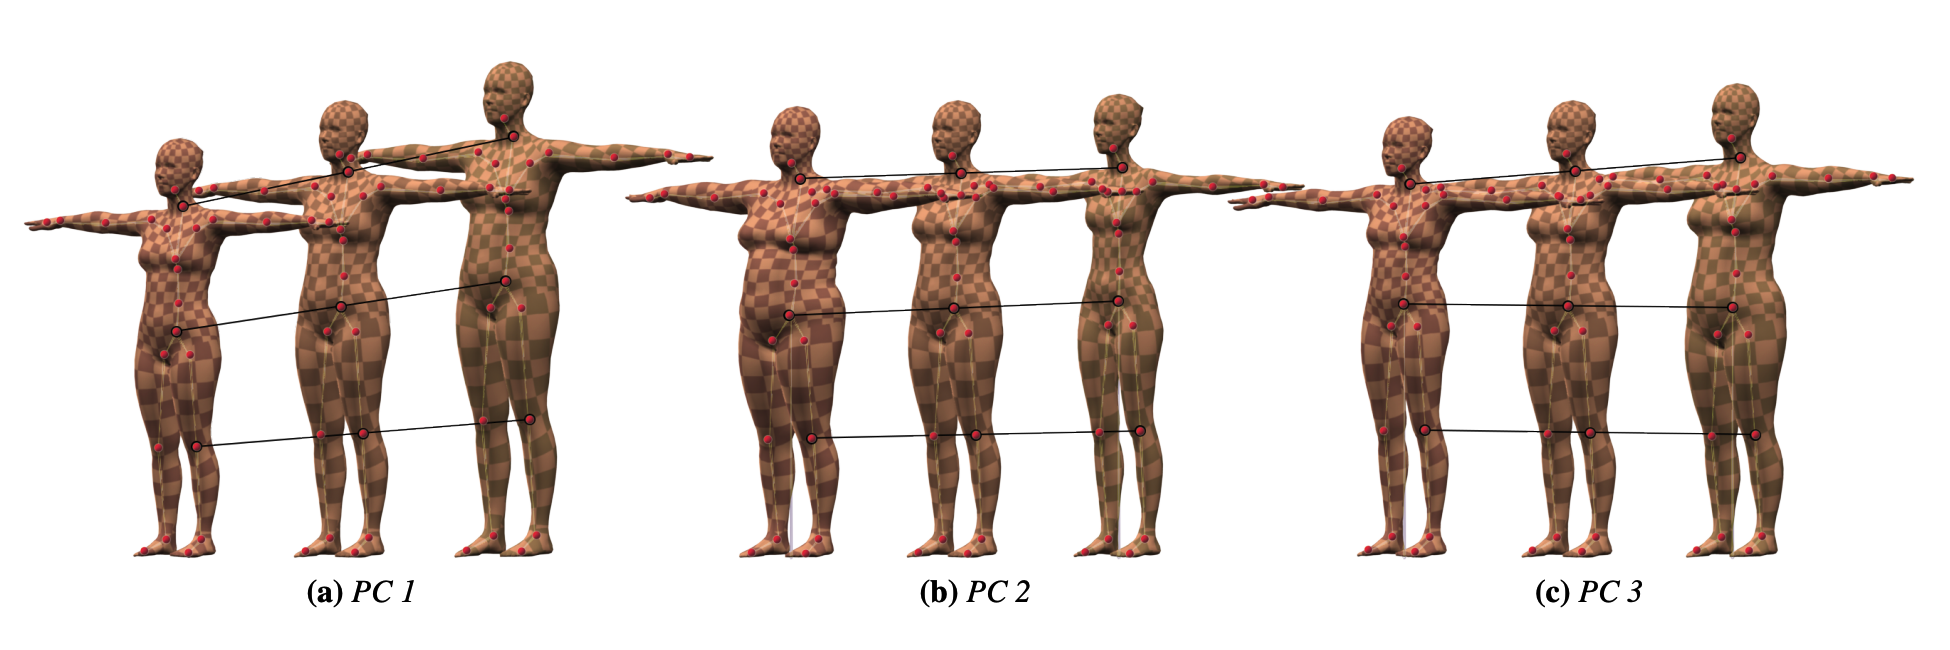
\includegraphics[width=0.9\textwidth]{figures/smpl_pc.png}
\caption{Prikaz prvih treh glavnih komponent oblike telesa ($PC1$, $PC2$ in $PC3$) modela SMPL~\cite{smpl}. Komponenti $PC1$ in $PC2$ sta prikazani v razponu $\pm 2$ standardnih odklonov, $PC3$ pa v razponu $\pm 5$ za boljšo vidnost variacije. Črne črte povezujejo istoležne sklepe med različnimi variacijami komponente in ponazarjajo njihov prostorski premik. Komponenta $PC1$ primarno določa višino telesa, $PC2$ maso, $PC3$ pa dolžino hrbtenice. Vir: Loper idr.~\cite{smpl}}
\label{fig:smpl_shape_pcs}
\end{figure}

Matematično je model definiran kot funkcija $M(\vec{\beta}, \vec{\theta})$, ki položaje oglišč izračuna skozi tri ključne korake, ki so opisani v nadaljevanju.

\subsubsection{Prilagoditev oblike in poze}
Postopek se začne z osnovno mrežo človeškega telesa v nevtralni pozi $\bar{T}$, ki se najprej prilagodi s premikom oblike (angl.\ \textit{shape displacement}) $B_S(\vec{\beta})$. Ta je definiran kot linearna kombinacija izračunanih glavnih komponent ${\mathcal{S} = [S_1, \dots, S_{|\vec{\beta}|}] \in \mathbb{R}^{3N \times |\vec{\beta}|}}$, kjer je $N$ število vozlišč mreže telesa:

$$B_S(\vec{\beta}; \mathcal{S}) = \sum_{k=1}^{|\vec{\beta}|} \beta_k S_k.$$

Nato se dodajo popravki zaradi poze $B_P(\vec{\theta})$, ki preprečujejo nezaželene artefakte pri upogibanju (npr. zmečkanje mreže v komolcu). Z $R(\vec{\theta}) \in \mathbb{R}^{9K}$ označimo vektor elementov rotacijskih matrik, ki ga dobimo tako, da elemente vseh rotacijskih matrik sklepov po vrsti zložimo v en sam vektor. Podobno z $R(\vec{\theta^*}) \in \mathbb{R}^{9K}$ označimo vektor elementov rotacijskih matrik za telo v nevtralni pozi. Popravke izračunamo kot:
$$B_P(\vec{\theta}; \mathcal{P}) = \sum_{n=1}^{9K} (R_n(\vec{\theta}) - R_n(\vec{\theta}^*)) P_n,$$
kjer je $P_n$ $n$-ti stolpec matrike $\mathcal{P} = [P_1, \dots, P_{9K}] \in \mathbb{R}^{3N \times 9K}$, ki vsebuje naučene korekcijske oblike telesa, $K$ pa je število sklepov telesa.

\subsubsection{Prilagoditev sklepov}
Lokacije sklepov $J(\vec{\beta})$ v modelu SMPL niso statične, temveč se morajo ujemati s telesno obliko, saj ima na primer višja oseba sklepe dlje narazen. Lokacije se izračunajo s pomočjo vnaprej naučenega linearnega regresorja $\mathcal{J}$ iz oglišč, ki so že prilagojena z obliko $\vec{\beta}$:
$$J(\vec{\beta}; \mathcal{J}, \bar{T}, \mathcal{S}) = \mathcal{J}(\bar{T} + B_S(\vec{\beta}; \mathcal{S})).$$

\subsubsection{Oblačenje}
\label{subsub:smpl_oblačenje}
V zadnji fazi se oglišča transformirajo v končno pozo z uporabo funkcije oblačenja $W$. Vsako oglišče $i$ se premakne na podlagi utežene kombinacije rotacij sosednjih sklepov:
$$M(\vec{\beta}, \vec{\theta}) = W(T_p(\vec{\beta}, \vec{\theta}), J(\vec{\beta}), \vec{\theta}, \mathcal{W}),$$
kjer je $T_p(\vec{\beta}, \vec{\theta}) = \bar{T} + B_S(\vec{\beta}) + B_P(\vec{\theta})$ mreža telesa s popravki, $\mathcal{W}$ pa so uteži oblačenja, ki določajo, kako močno posamezen sklep vpliva na premik določenega oglišča telesa.


\section{Podatkovna množica AMASS}
\label{sec:amass}
AMASS (angl.\ \textit{Archive of Motion Capture as Surface Shapes}) je obsežen arhiv podatkov o gibanju ljudi, ki v enotnem formatu združuje 15 različnih množic podatkov optičnega zajema gibanja (angl. \textit{motion capture} oziroma mocap), kot so CMU, KIT in HumanEva. Glavni izziv pri združevanju teh baz je uporaba različnih naborov markerjev in specifičnih protokolov. AMASS ta problem rešuje z uporabo metode MoSh++, ki podatke različnih vrst preslika v skupen parametrični prostor modelov SMPL-H~\cite{smplh} in DMPL, ki sta razširitvi modela SMPL. V nasprotju s tradicionalnimi metodami mocap, ki ocenjujejo le položaje sklepov skeleta, AMASS omogoča rekonstrukcijo celotne 3D mreže človeškega telesa v vsakem časovnem okvirju. Kot je prikazano na sliki \ref{fig:amass_mosh}, MoSh++ zajame poze, obliko telesa in dinamične deformacije mehkih tkiv (npr.\ tresenje mišic in maščobnih tkiv med gibanjem).

\begin{figure}[h]
\centering
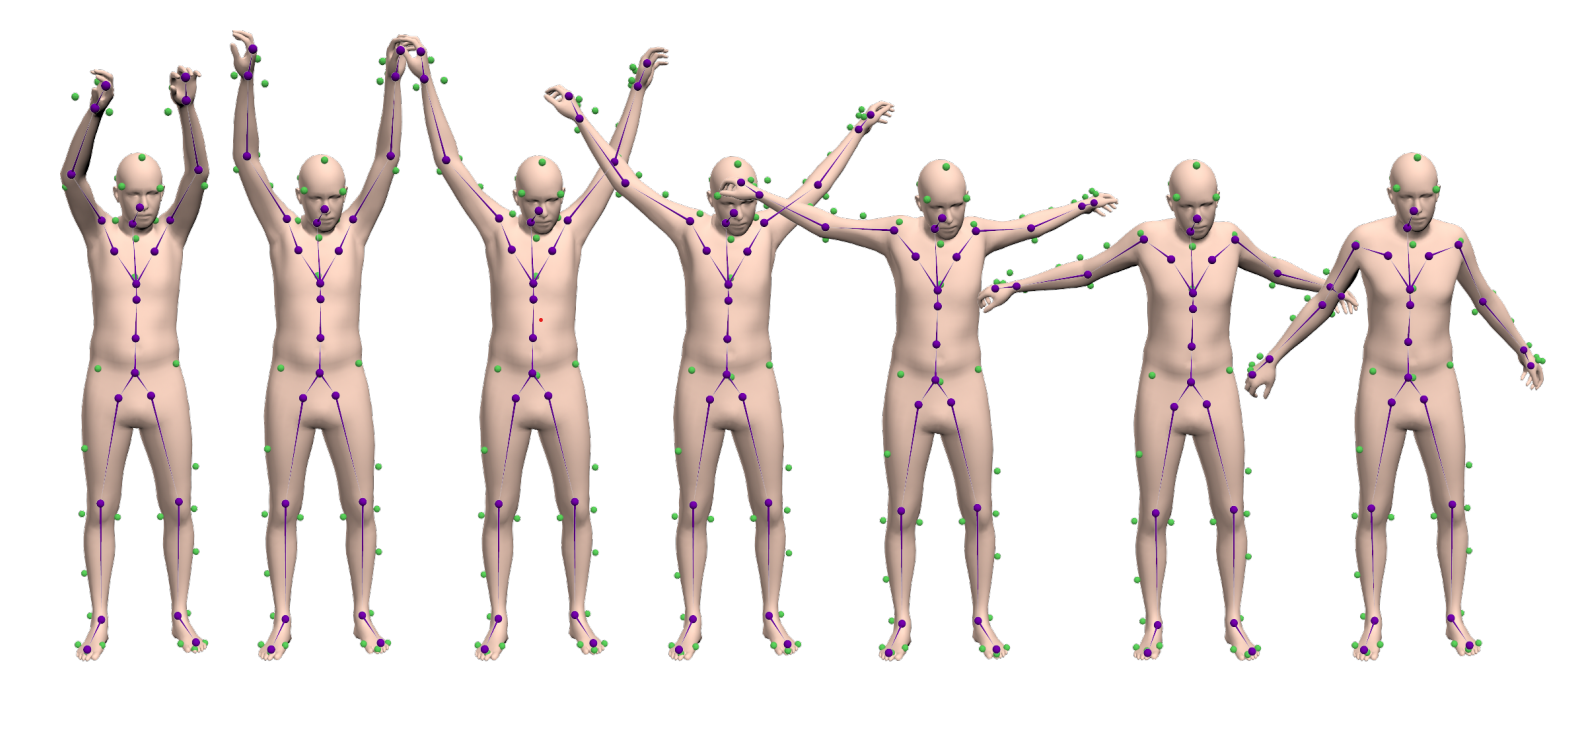
\includegraphics[width=0.8\textwidth]{figures/amass_mosh.png}
\caption{Primerjava med tradicionalnim zajemom gibanja in metodo MoSh++ v zbirki AMASS~\cite{amass}. Tradicionalne metode (vijolično) aproksimirajo le skelet, medtem ko lahko MoSh++ s parametri modelov SMPL-H in DMPL (zeleno) predstavi obliko telesa in dinamiko mehkih tkiv. Vir: Mahmood idr.~\cite{amass}}
\label{fig:amass_mosh}
\end{figure}

Zbirka AMASS vključuje več kot 40 ur podatkov o gibanju, ki zajemajo več kot 300 subjektov in 11.000 posnetkov. Vsak časovni okvir v zbirki je določen z naslednjimi parametri:

\begin{itemize}
\item \textbf{Parametri oblike $\vec{\beta}$}: 16 komponent PCA za določitev oblike telesa.
\item \textbf{Parametri poze $\vec{\theta}$}: 159 komponent, ki določajo celotno kinematično konfiguracijo telesa in dlani v prostoru. Dekompozicija teh parametrov obsega:

\begin{itemize}
\item \textbf{globalno translacijo} telesa v prostoru (3 parametri),
\item \textbf{rotacije 22 telesnih sklepov} ($22 \times 3 = 66$ parametrov), ki določajo pozo trupa in udov, ter
\item \textbf{rotacije 30 sklepov dlani} ($30 \times 3 = 90$ parametrov), ki določajo postavitev dlani.
\end{itemize}

\item \textbf{Parametri mehkih tkiv $\vec{\phi}$}: 8 komponent modela DMPL za modeliranje tresenja mišic in maščobnih tkiv.
\end{itemize}

Matematično AMASS razširi funkcijo oblačenja, predstavljeno v poglavju \ref{subsub:smpl_oblačenje}, s členom za dinamične popravke $B_D(\vec{\phi})$, ki so bili naučeni iz 4D skenov ljudi v gibanju. Osnovna mreža človeškega telesa v nevtralni pozi $\bar{T}$, se sedaj popravi s tremi členi:
$$T_p(\vec{\beta}, \vec{\theta}, \vec{\phi}) = \bar{T} + B_S(\vec{\beta}) + B_P(\vec{\theta}) + B_D(\vec{\phi}).$$

Končna oblika mreže telesa $S(\vec{\beta}, \vec{\theta}, \vec{\phi})$ je tako definirana kot:


$$S(\vec{\beta}, \vec{\theta}, \vec{\phi}) = G(T_p(\vec{\beta}, \vec{\theta}, \vec{\phi}), J(\vec{\beta}), \vec{\theta}, \mathcal{W}).$$

Zaradi svoje enotne predstavitve in velikega obsega je AMASS postal ključni vir za učenje in ovrednotenje modelov globokega učenja za simulacijo tkanin. V tej nalogi sekvence iz AMASS služijo kot standardiziran vir gibanja, ki zagotavlja, da primerjava med modeli temelji na fizikalno smiselnih in raznolikih položajih telesa.


\section{Metrike za primerjavo simulacij}
V tem poglavju opišemo metrike, ki smo jih uporabili za analizo modelov. Te metrike ocenjujejo geometrijsko natančnost, časovno stabilnost in fizikalno konsistentnost napovedi nevronskega modela v primerjavi z referenčno fizikalno osnovano simulacijo. V nadaljevanju je za vsako metriko opisan izračun na ravni posameznega
časovnega okvirja sekvence.

\subsubsection{Korenska srednja kvadratna napaka}
Za ocenjevanje prostorske natančnosti smo uporabili korensko srednjo kvadratno napako (angl.\ \textit{Root Mean Square Error}, RMSE). Ta metrika oceni, kakšna je povprečna evklidska razdalja med napovedanimi položaji oglišč $\hat{v}_i$ in referenčnimi položaji $v_i$:
$$RMSE = \sqrt{\frac{1}{N} \sum_{i=1}^{N} ||v_i - \hat{v}_i||^2},$$
kjer $N$ predstavlja število oglišč v mreži oblačila. RMSE močneje penalizira večja odstopanja v geometriji, kar je koristno za prepoznavanje večjih odstopanj tkanine.

\subsubsection{Napaka pospeška}
Časovno gladkost simulacije smo ovrednotili z napako pospeška oglišč. Ta metrika je ključna za prepoznavanje vizualnega migotanja, ki se pogosto pojavi pri nevronskih mre\-žah, ki ne upoštevajo časovne odvisnosti. Diskretni pospešek oglišča $i$ v trenutku $t$ se določi s pomočjo položajev $x_i$ v treh zaporednih časovnih okvirih:
$$a_i^t = x_i^{t-1} - 2x_i^t + x_i^{t+1}.$$
Vektorje pospeška izračunamo za predikcijo modela ter za referenčno simulacijo. Napaka pospeška $E_{acc}^t$ je nato definirana kot povprečna evklidska razdalja med temi vektorji:
$$E_{acc}^t = \frac{1}{N} \sum_{i=1}^{N} \|a_i^t - \hat{a}_i^t\|,$$
kjer $N$ predstavlja število oglišč, $t$ trenutni časovni okvir, ${a}_i^t$ referenčni pospešek, $\hat{a}_i^t$ pa napovedani pospešek. S to metriko kvantificiramo, koliko fizikalne vztrajnosti model dejansko ohranja.

\subsubsection{Delež kolizij}
Delež kolizij meri stopnjo prodiranja mreže tkanine v mrežo telesa. Ker imata telo in oblačilo na tisoče oglišč, smo za učinkovito iskanje oglišč v mrežah uporabili podatkovno strukturo KD-drevesa, ki omogoča iskanje najbližjih sosedov v prostoru s časovno zahtevnostjo $O(\log N)$. Postopek določanja kolizije za vsako posamezno oglišče tkanine $c_i$ se izvede v naslednjih korakih:

\begin{enumerate}
\item \textbf{Iskanje najbližjega soseda}: S pomočjo KD-drevesa poiščemo oglišče telesa $b_i$, ki je prostorsko najbližje oglišču tkanine $c_i$.
\item \textbf{Izračun vektorja razdalje}: Določimo vektor $\vec{d_i}$ od najdenega oglišča na telesu do oglišča na tkanini:
$$\vec{d_i} = c_i - b_i.$$
\item \textbf{Preverjanje s skalarnim produktom}: Izračunamo skalarni produkt med vektorjem razdalje in normalo površine telesa $\vec{n}_i$ v točki $b_i$:
$$s_i = \vec{d_i} \cdot \vec{n}_i.$$
\end{enumerate}

Kot je prikazano na sliki~\ref{fig:collision_dot_product}, nam vrednost skalarnega produkta $s_i$ pove, kje v prostoru se nahaja oglišče tkanine glede na normalo oglišča telesa:

\begin{itemize}
\item Če je $s_i < 0$, vektor $\vec{d_i}$ kaže v nasprotno smer od normale $\vec{n}_i$, kar pomeni, da je oglišče tkanine prodrlo v notranjost telesa.
\item Če je $s_i \ge 0$, se oglišče nahaja na površini ali zunaj telesa, torej ni prišlo do kolizije.
\end{itemize}

Celotni delež kolizij $C_{rate}$ smo določili kot razmerje med številom vseh penetracij in skupnim številom oglišč oblačila:
$$C_{rate} = \frac{\sum\limits_{s_i < 0}1}{N}.$$

\begin{figure}[h]
\centering
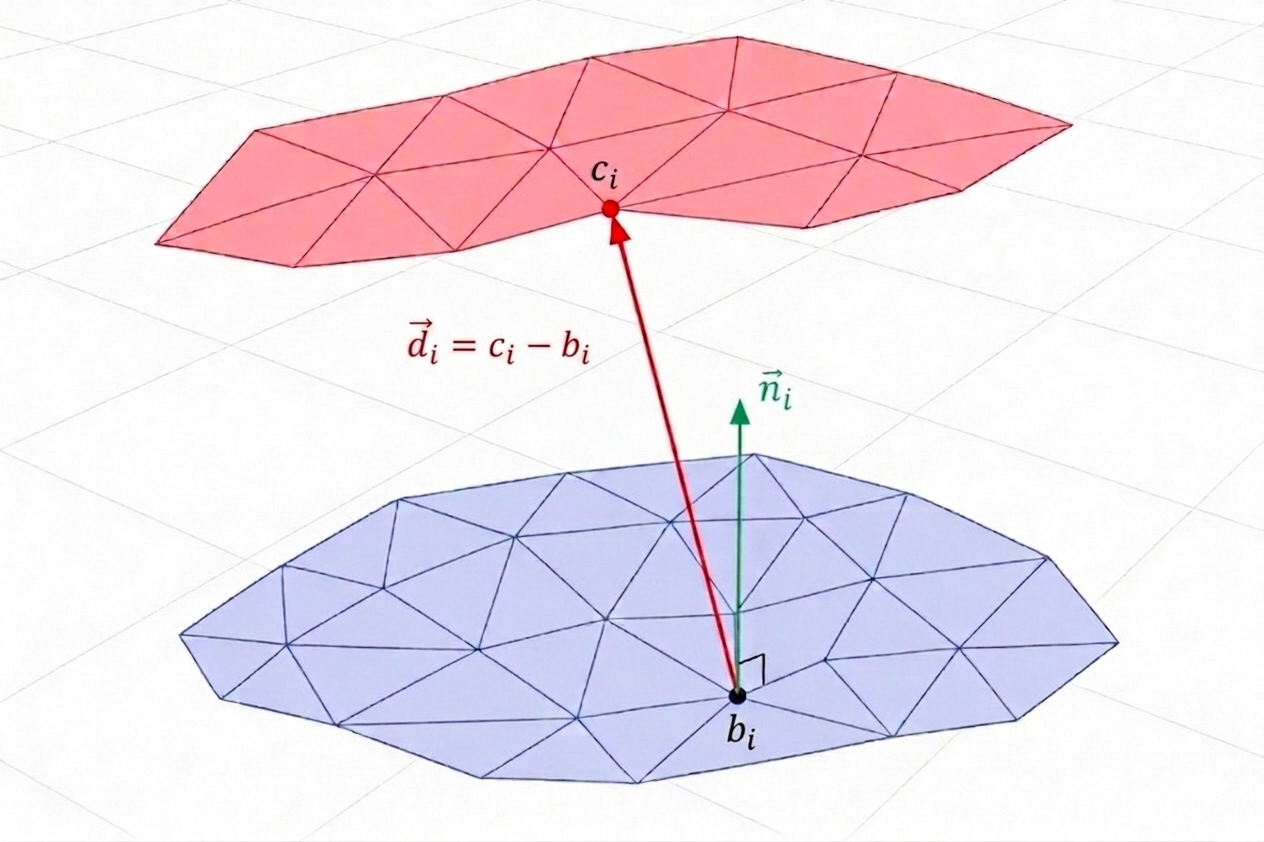
\includegraphics[width=0.8\textwidth]{figures/collision_dot_product.png}
\caption{Geometrijski prikaz določanja kolizije s skalarnim produktom. Vektor $\vec{d_i}$ kaže od opazovanega oglišča telesa (modro) do najbližega oglišča tkanine (rdeče). Negativen skalarni produkt z normalo $\vec{n_i}$ nakazuje, da je oglišče tkanine prodrlo pod površino telesa.}
\label{fig:collision_dot_product}
\end{figure}



%----------------------------------------------------------------
% Poglavje (Chapter) 4
%----------------------------------------------------------------
\chapter{Primerjalna analiza modelov}
\label{ch:primerjalna_analiza_modelov}

V tem poglavju predstavimo eksperimentalno okolje, pripravo vhodnih podatkov in primerjalni cevovod, s katerim smo ovrednotili izbrane modele simulacije tkanine. Najprej opišemo uporabljene sekvence gibanja, standardizacijo geometrije in pripravo referenčne simulacije, nato pa podamo še rezultate primerjalne analize ter utemeljimo izbiro modela za mobilno implementacijo.

\section{Eksperimentalno okolje}
Vse simulacije,  meritve in analize modelov smo izvedli v enem računalniškem okolju, do katerega smo dostopali preko oddaljenega namizja. To napravo smo izbrali, ker omogoča hitro izvajanje simulacij na grafični procesni enoti (GPE). Vsebovala je dva procesorja Intel(R) Xeon(R) Gold 6140 CPU @ 2.30GHz z 18 fizičnimi jedri in 36 procesnimi nitmi. Vgrajeni sta tudi dve grafični kartici NVIDIA RTX 4000 Ada, ki omogočata polno strojno pospeševanje v okolju CUDA.

\subsubsection{Podatkovna množica AMASS in izbor subjektov}
Za pridobitev realističnih in raznolikih podatkov o gibanju smo uporabili arhiv AMASS, opisan v poglavju \ref{sec:amass}. Da bi zagotovili variabilnost telesnih konstitucij, smo izbrali štiri različne moške subjekte z identifikatorji 01, 02, 05 in 07. Za vsakega posameznika smo izbrali pet različnih sekvenc gibanja (indeksi od 01 do 05), kar skupno predstavlja 20 unikatnih posnetkov. Izbrane sekvence pokrivajo širok nabor človeškega gibanja, kar je pomembno za testiranje stabilnosti simulacij pri raznolikih gibih.

Zaradi visoke računske zahtevnosti in preprečevanja kombinatorične eksplozije smo se omejili na moški model telesa. Kljub tej omejitvi je načrt eksperimentov dovolj obsežen, saj vključuje:

\begin{itemize}
\item 3 tipe oblačil: majico s kratkimi rokavi (t-shirt), srajco (shirt) in hlače (pants).
\item 2 tipa materialov: bombaž in svila.
\end{itemize}

Za vsako od 20 sekvenc gibanja smo izvedli simulacije z vsemi kombinacijami treh tipov oblačil. Pri modelih HOOD, ContourCraft in Maya nCloth smo uporabili oba materiala, torej 6 unikatnih oblačil, medtem ko smo pri modelu TailorNet zaradi omejitev arhitekture simulirali le bombaž, torej imamo le 3 unikatna oblačila. Skupno smo tako analizirali 420 simulacij ($20*6 + 20*6 + 20*6 + 20*3$) izvedenih na GPE, kar je dobra statistična osnova za primerjavo metod.


\section{Priprava geometrije oblačil}
Eden največjih izzivov pri primerjavi modelov TailorNet~\cite{TailorNet}, HOOD~\cite{hood} in ContourCraft~\cite{contourcraft} je, kako zagotoviti testiranje na enotni podatkovni množici, saj modeli sprejemajo zelo različne vrste podatkov. Da zagotovimo objektivne pogoje testiranja, moramo ustvariti ločene cevovode priprave podatkov za vsak model posebej, ki bodo mreže oblačil in teles prilagodili na pričakovan format vhodnih podatkov.

\subsubsection{Unifikacija mrež in pretvorba formatov}
Model TailorNet je naučen na specifičnih kategorijah oblačil (majica, srajca, hlače, ...), zato smo njegovo podatkovno množico oblačil uporabili kot skupni imenovalec za vse testirane modele. Ker pa modeli za svoje delovanje zahtevajo različne strukture podatkov, smo izvedli naslednje pretvorbe:

\begin{itemize}
\item \textbf{TailorNet}: Vhodni podatki so shranjeni v formatu \texttt{.npy}, ki vsebuje informacije o ogliščih in topologiji.
\item \textbf{HOOD in ContourCraft}: Iz TailorNet geometrije smo z uporabo skripte \textit{GarmentCreator}, ki je dostopna v repozitoriju HOOD in ContourCraft, ustvarili mreže in pripadajoče metapodatke v formatu \texttt{.pkl}. Slovar v tej datoteki vključuje tudi podatke o sosednosti oglišč, kar je nujno za delovanje nevronskih mrež nad grafi.
\item \textbf{Maya}: Iz TailorNet predlog oblačil smo izvozili standardne datoteke \texttt{.obj}, ki služijo kot vhodna geometrija za nCloth reševalnik.
\end{itemize}

\subsubsection{Optimizacija parametrov oblike in stila}
Vsako oblačilo v naši primerjavi določata dva nabora parametrov: $\beta$ (oblika telesa, npr. širina ramen, obseg pasu, dolžina nog,...) in $\gamma$ (slog oblačila, npr. dolžina rokavov, oprijetost, dolžina hlačnic,...). Ker so modeli teles iz baze AMASS zelo raznoliki, smo za vsakega od 4 subjektov posebej poiskali ustrezne parametre za vsak tip oblačila. Za vsak poizkus nabora parametrov smo vizualizirali prileganje oblačila telesu v nevtralni pozi. Cilj je najti takšne vrednosti parametrov, kjer oblačilo tesno objame telo, ne da bi prišlo do neželenih začetnih penetracij ali prevelikih razmakov, ki bi popačili rezultate simulacij.

\subsubsection{Reševanje začetnih kolizij}
Eden izmed izzivov pri standardizaciji vhodnih podatkov je bilo neujemanje nevtralnih (kanoničnih) poz med modeli. Surove poze iz baze AMASS~\cite{amass} lahko vsebujejo samopresekanja mrež v predelu ramen in pazduh. Če oblačilo inicializiramo neposredno v takšno pozo, bi se rokavi že v začetnem okvirju nahajali znotraj telesa, kar bi povzročilo nestabilnost simulacije.

Pri prilagajanju mrež smo ugotovili, da TailorNet~\cite{TailorNet} shranjuje oblačila v nevtralni A-pozi, medtem ko arhitekturi HOOD~\cite{hood} in ContourCraft~\cite{contourcraft} pričakujeta vhodno mrežo v T-pozi. Zaradi te razlike so pri neposrednem prenosu rokavi majic segali prenizko in prodirali skozi roke telesa, kot je prikazano na sliki~\ref{fig:pose_mismatch}. Težavo smo odpravili s transformacijo TailorNetovih oblačil v T-pozo s pomočjo orodij znotraj TailorNet repozitorija.

Za vse modele smo dodatno uporabili še logiko razmikanja rok, ki poveča kot med torzom in rokami. V prvem okvirju smo spremenili rotacijo ramenskih sklepov, tako da smo spremenili rotacijske parametre poze $\theta$. To logiko, ki je izvorno prisotna v ogrodjih HOOD in ContourCraft, smo implementirali še za TailorNet in simulacijo v Mayi. S tem smo zagotovili, da ima tkanina dovolj prostora za začetek simulacije in so pogoji za vse simulacije enakovredni.

\begin{figure}[h]
\centering
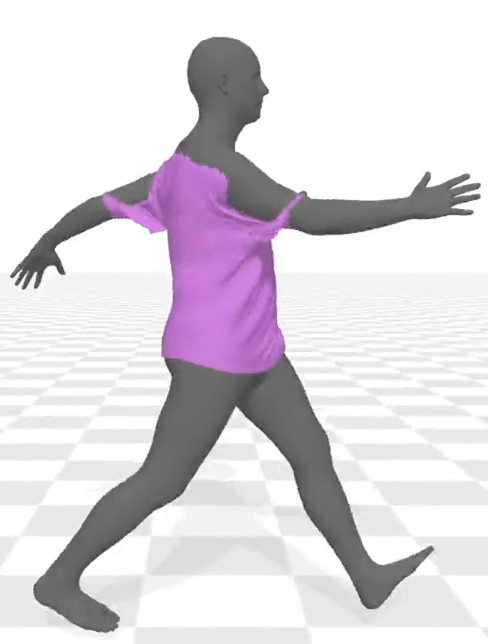
\includegraphics[width=0.4\textwidth]{figures/pose_mismatch.png}
\caption{Vizualizacija napake pri prenosu oblačila na ContourCraft: rokavi TailorNet majice prodirajo skozi mrežo telesa zaradi neujemanja med pričakovanimi začetnimi pozami.}
\label{fig:pose_mismatch}
\end{figure}


\section{Referenčna simulacija v orodju Maya}
Za generiranje prave vrednosti simulacije (angl.\ \textit{ground truth}) smo uporabili Mayin fizikalni simulator nCloth~\cite{maya_ncloth}, ki temelji na metodi delcev in vzmeti. Celoten postopek smo avtomatizirali s skriptnim cevovodom nCloth\_sim.py, da smo zagotovili konsistentnost med različnimi sekvencami gibanja.

\subsubsection{Model telesa kot kolizijsko telo}
V vsaki simulaciji smo uporabili gibanje iz arhiva AMASS~\cite{amass} kot neposreden vir animacije. Iz parametrov SMPL~\cite{smpl} smo izluščili oglišča in ploskve telesa, ki smo jih v Mayo uvozili kot mrežo v \textit{.obj} formatu. To mrežo smo določili kot pasivno kolizijsko telo, ki med simulacijo fizikalno vpliva na premikanje tkanine oblačila. Da smo zagotovili popolno časovno usklajenost z izhodi nevronskih mrež, smo v cevovod vsilili ciljno število sličic na sekundo (angl.\ \textit{Frames per second}), ki se ujema s frekvenco vzorčenja modelov v bazi AMASS.

\subsubsection{Fizikalne lastnosti materialov}
Za simulacijo različnih vrst blaga smo izbrali specifične fizikalne parametre. Osredotočili smo se na bombaž in svilo. Parametre smo določili ročno na podlagi vizualne ocene simulacije. Vrednosti smo prilagajali tako, da je gibanje tkanine čim bolj ustrezalo pričakovanemu obnašanju materiala, ki smo ga želeli simulirati. Za vsak material v nCloth reševalniku smo nastavili naslednje lastnosti:

\begin{itemize}
\item masa in trenje površine,
\item odpornost na raztezanje, stiskanje in upogibanje,
\item dušenje gibanja (angl.\ \textit{damping}),
\item debelina tkanine in debelina kolizijskega roba.
\end{itemize}

Te nastavitve omogočajo, da se referenčna simulacija vizualno in fizikalno odziva skladno z naravo uporabljenega materiala. Točne vrednosti uporabljenih parametrov so navedene v izvorni kodi simulacijskega postopka.

\subsubsection{Pripenjanje oglišč}
Da oblačila med gibanjem ne padejo s telesa, smo implementirali logiko pripenjanja oglišč na kolizijsko telo. Pri zgornjih delih oblačil (majica, srajca) smo fiksirali zgornja 2\,\% oglišč (predvsem okoli ovratnika), pri hlačah pa zgornjih 10\,\% oglišč (predel pasu). Ta delež oglišč togo sledi gibanju telesa, preostali del mreže pa je prepuščen prosti fizikalni simulaciji. Enako logiko pripenjanja smo uporabili pri vseh testiranih nevronskih modelih.


\section{Implementacija primerjalnega cevovoda}
Zaradi heterogenosti uporabljenih modelov smo morali razviti sistem za ekstrakcijo in standardizacijo podatkov. Ker je vsak model temeljil na drugačnih podatkovnih strukturah, smo se odločili za primerjavo rezultatov na nivoju izvoženih geometrijskih mrež, namesto neposredne primerjave tenzorjev inference.

\subsubsection{Ekstrakcija in standardizacija uvoza}
Izhode modelov HOOD in ContourCraft, ki so bili shranjeni v paketih rezultatov formata \texttt{.pkl}, smo pretvorili v začasne datoteke \texttt{.obj}. Podoben postopek smo uporabili za rezultate modela TailorNet, ki so bili prvotno v formatu \texttt{.ply}. Ker smo mreže želeli vizualizirati v Mayi, nam je ta pristop olajšal postopek, saj se je uporaba ukazov \texttt{cmds} za uvoz zunanjih datotek izkazala za bistveno hitrejšo in stabilnejšo od neposrednega generiranja mrež preko ogrodja OpenMaya.

Da bi preverili pravilnost generiranih mrež in ali so med seboj pravilno poravnane, smo implementirali skripto za vzporedni pregled vseh štirih metod v eni sceni v Mayi. Primer take scene je prikazan na sliki \ref{fig:maya_results}. Ko smo rezultate vizualizirali, smo opazili napako v poravnavi osi pri modelu TailorNet. Ugotovili smo, da je koordinatni sistem usmerjen z Z-osjo navzgor, medtem ko imajo Maya in preostali uporabljeni modeli Y-os usmerjeno navzgor. Neskladje smo odpravili z uvedbo eksplicitne rotacije rezultatov vseh TailorNetovih mrež, s čimer smo zagotovili pravilno pokončno orientacijo teles ob uvozu.

Natančna primerjava med metodami pa potrebuje več kot le enako usmeritev koordinatnih sistemov rezultatov. Za izračun metrik morajo biti rezultati popolnoma poravnani med sabo v prostoru. Čeprav smo predhodno uredili globalno orientacijo, so v podatkih še vedno ostajala manjša prostorska odstopanja. Za odpravo teh razlik smo uporabili algoritem iterativne najbližje točke (angl.\ \textit{Iterative Closest Point}, ICP).

Kot referenčno telo smo določili mrežo telesa, generirano v okolju Maya. Postopek smo zasnovali tako, da je algoritem najprej poiskal optimalno transformacijo za oglišča telesa testiranega modela glede na referenco. To transformacijsko matriko smo uporabili še za pripadajočo mrežo oblačila. To je ohranilo medsebojni odnos obeh elementov in zagotovilo, da so bili vsi modeli v koordinatnem sistemu Maye poravnani z milimetrsko natančnostjo. Takšna standardizacija prostora je bila ključna, da smo lahko kasneje vse izmerjene napake pripisali dejanskim razlikam v simulaciji in ne napakam pri uvozu podatkov.

Pri uporabi algoritma ICP smo izvedli še optimizacijo, ker bi bila natančna poravnava na celotnih gostih mrežah prepočasna za obdelavo tako velikega števila simulacij. V postopku smo uporabili naključno podvzorčenje in s tem zmanjšali število točk, uporabljenih za izračun transformacijske matrike. Preverili smo, da pri tem nismo opazno izgubili natančnosti same poravnave.

\begin{figure}[h]
\centering
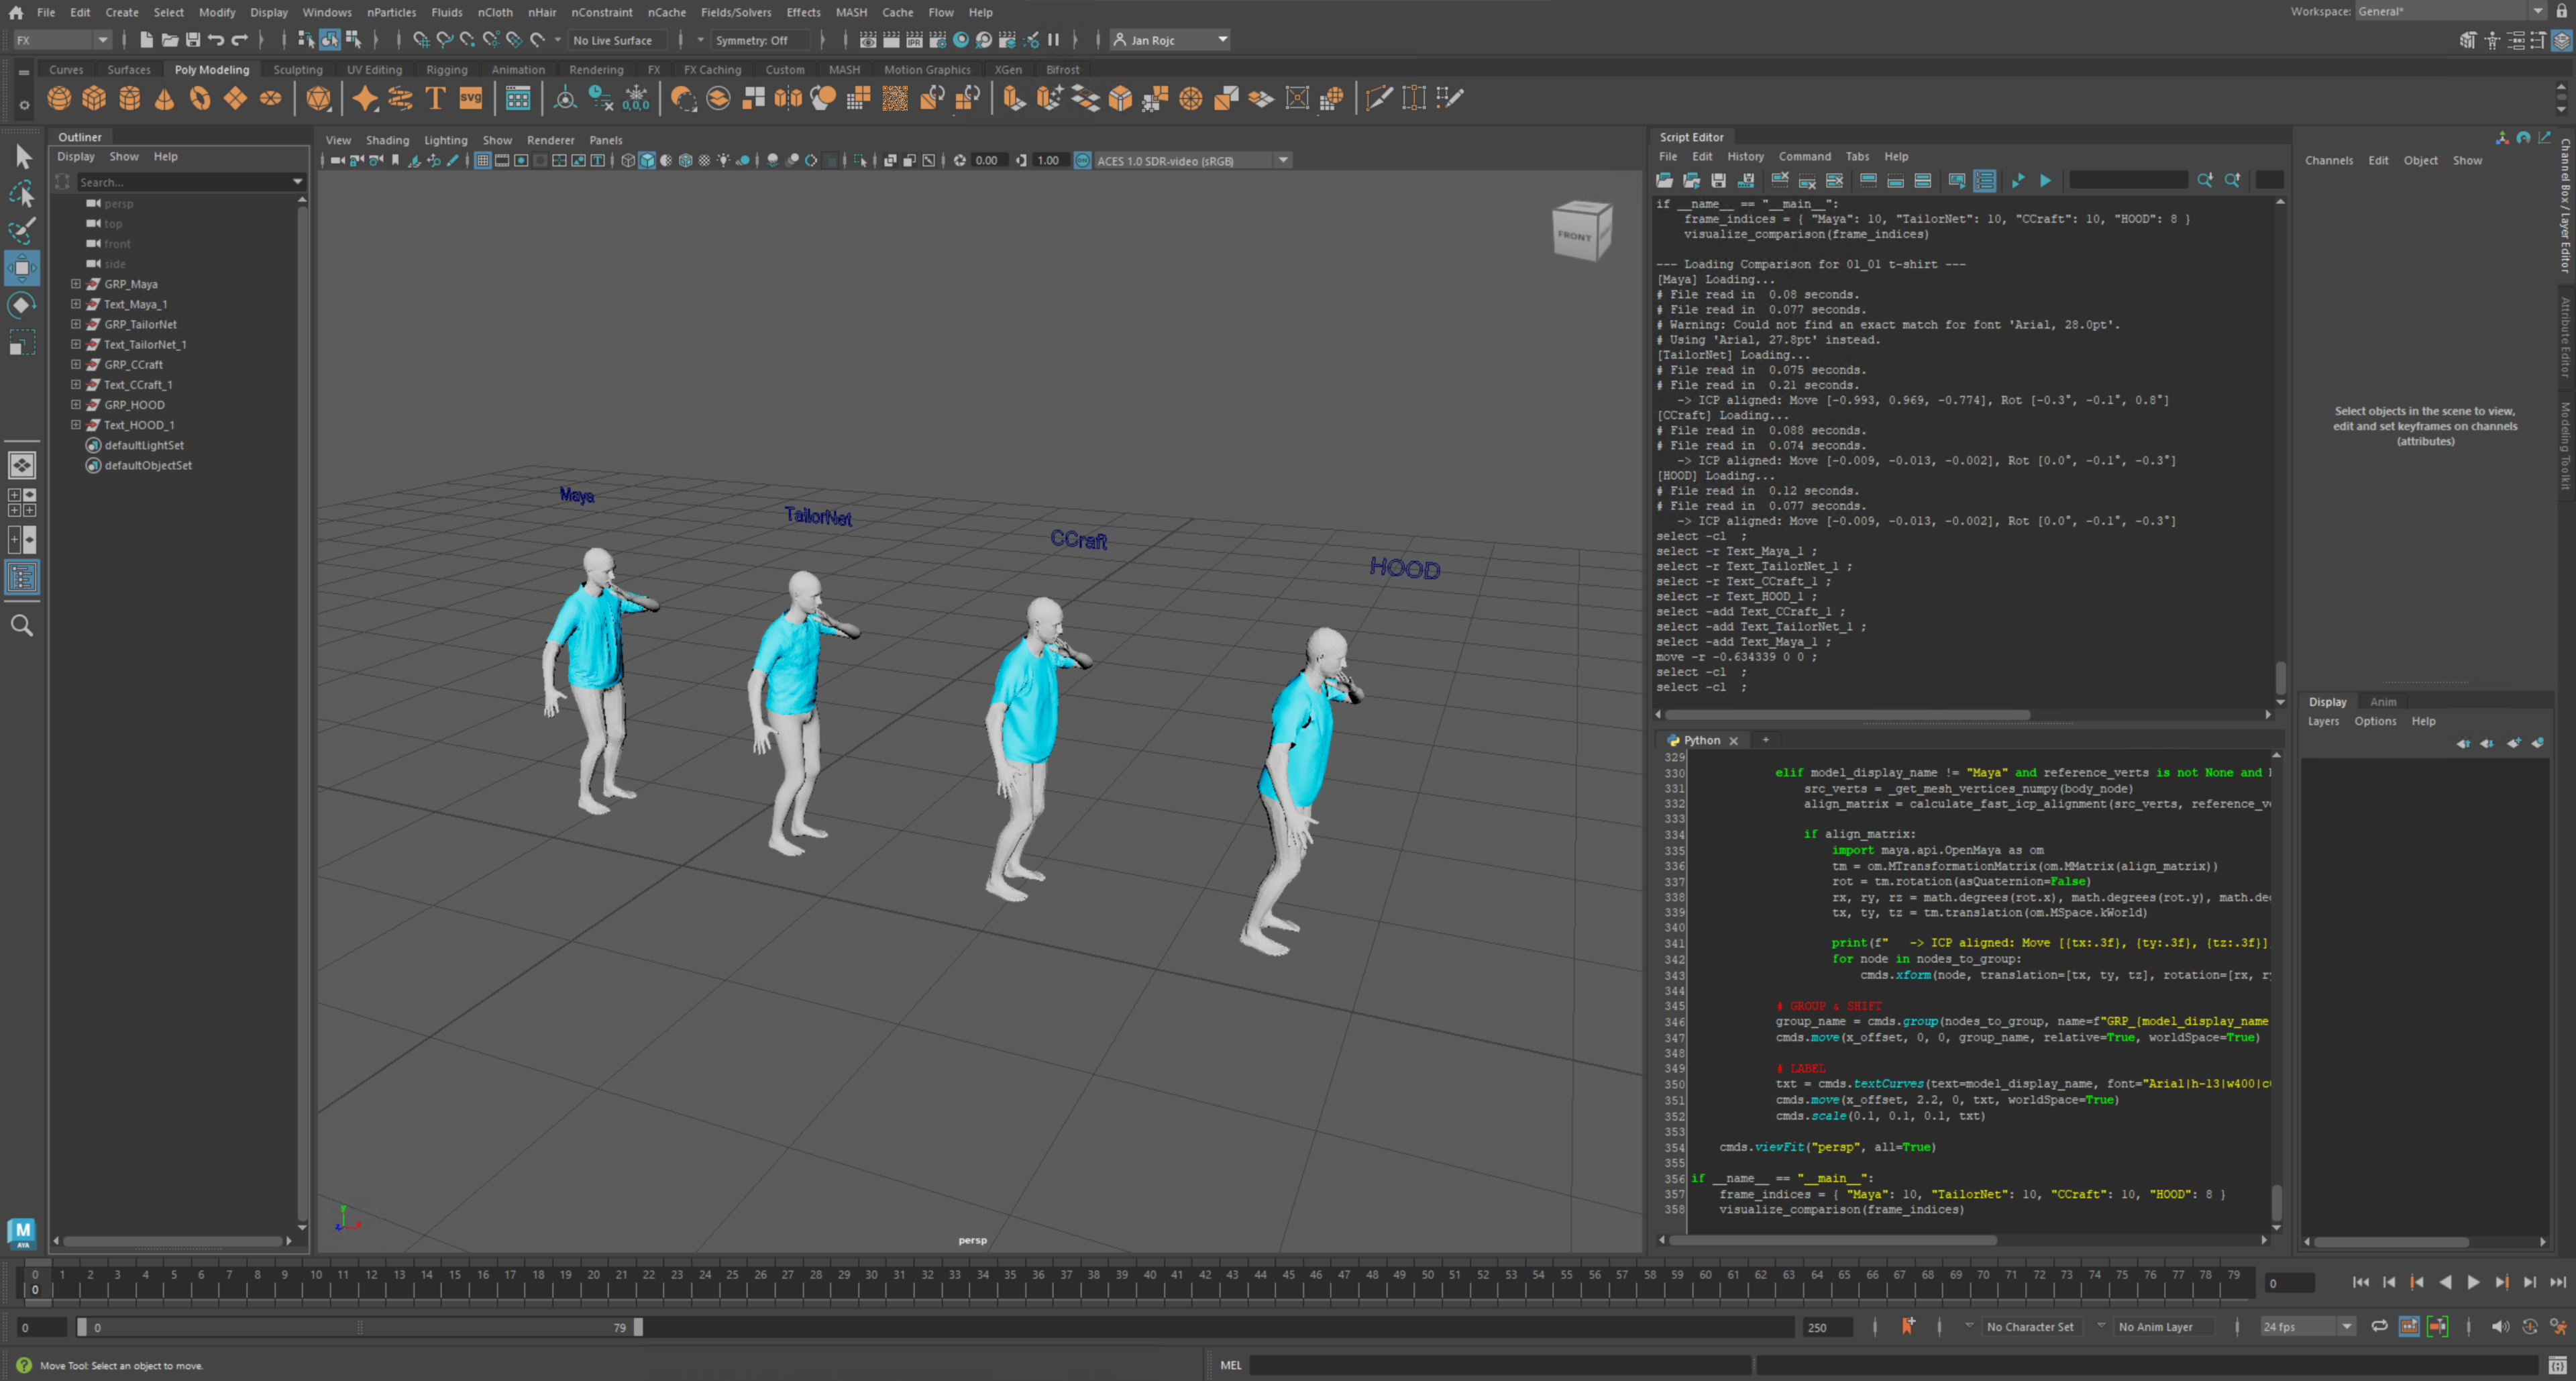
\includegraphics[width=1\textwidth]{figures/maya_results.png}
\caption{Avtomatizirana vizualizacija rezultatov vseh 4 modelov v eni sceni v programski opremi Maya.}
\label{fig:maya_results}
\end{figure}

\subsubsection{Rezultati in primerjalna analiza}
Po izvedbi vseh $420$ simulacij in geometrijski poravnavi mrež smo začeli z analizo pridobljenih podatkov. Rezultate smo obdelali v dveh korakih: najprej smo izračunali povprečne vrednosti metrik čez vse časovne okvirje posamezne sekvence, nato pa te vrednosti ponovno povprečili čez celoten nabor sekvenc, da smo pridobili globalno oceno uspešnosti posameznega modela. Kot prikazuje tabela~\ref{tab:global_results}, sta modela HOOD in ContourCraft dosegla skoraj trikrat nižji RMSE in več kot šestkrat nižjo napako pospeška v primerjavi s TailorNetom. Še bolj izrazita razlika se je pokazala pri deležu kolizij, kjer je TailorNet dosegel $6,29\,\%$, medtem ko sta grafna modela delež trkov zadržala pod $1\,\%$. Za bolj natančno predstavo o porazdelitvi smo podatke prikazali z diagramom s škatlo z brki na sliki \ref{fig:metrics_box_plots}.

\begin{table}[h]
\centering
\begin{tabular}{lccc}
\hline
\textbf{Model} & \textbf{RMSE (m)} & \textbf{Napaka pospeška} & \textbf{Delež kolizij ($\%$)} \\
\hline
TailorNet & $0,103 \pm 0,16$ & $0,017 \pm 0,03$ & $6,287 \pm 3,56$ \\
ContourCraft & $0,039 \pm 0,01$ & $0,003 \pm 0,01$ & $0,595 \pm 0,91$ \\
HOOD & $0,035 \pm 0,01$ & $0,003 \pm 0,01$ & $0,910 \pm 1,26$ \\ \hline
\end{tabular}
\caption{Globalni rezultati natančnosti za bombažne materiale s pripadajočimi standardnimi odkloni.}
\label{tab:global_results}
\end{table}

Da bi preverili robustnost modelov za različne tipe oblačil, smo RMSE rezultate izračunali tudi za vsak tip posebej in jih izpisali v tabelo ~\ref{tab:clothing_types_results}. Hlače so predstavljale največji izziv za model TailorNet, kjer je RMSE narasel na $0,128$ z višjim standardnim odklonom. Pri modelih HOOD in ContourCraft pa so bili rezultati bistveno bolj konsistentni čez vse kategorije. Pri srajcah in kratkih majicah sta oba grafna modela ohranila RMSE pod $0,041$, kar potrjuje njuno robustnost pri različnih topologijah oblačil.

\begin{table}[h]
\centering
\begin{tabular}{lccc}
\hline
\textbf{Model} & \textbf{Kratka majica} & \textbf{Srajca} & \textbf{Hlače} \\
\hline
TailorNet & $0,086 \pm 0,09$ & $0,094 \pm 0,10$ & $0,128 \pm 0,24$ \\
ContourCraft & $0,041 \pm 0,01$ & $0,037 \pm 0,01$ & $0,038 \pm 0,02$ \\
HOOD & $0,037 \pm 0,001$ & $0,035 \pm 0,01$ & $0,033 \pm 0,02$ \\ \hline
\end{tabular}
\caption{Globalni rezultati RMSE segmentirani po tipu oblačila s pripadajočimi standardnimi odkloni.}
\label{tab:clothing_types_results}
\end{table}

Pri analizi vpliva materialov smo ugotovili, da svila zaradi svoje narave (večje število gub in nižja togost) povzroča nekoliko višje napake v vseh kategorijah. RMSE se je pri modelu HOOD z $0,0352$ pri bombažu povišal na $0,0381$ pri svili, podoben trend pa smo opazili tudi pri napaki pospeška. Ker TailorNet ne omogoča neposrednega spreminjanja fizikalnih parametrov do te mere, da bi simulirali svilo, so ti podatki na voljo le za preostala modela. Kljub zahtevnosti materiala sta HOOD in ContourCraft ohranila delež kolizij pod $1\,\%$. Ker so dvojna povprečenja (najprej čez posamezne okvirje in nato čez celotne sekvence) statistično nevarna, saj nanje osamelci močno vplivajo, smo porazdelitve metrik čez vse sekvence dodatno vizualizirali z diagrami s škatlo z brki, ločeno za bombaž in svilo. Kot vidimo na sliki \ref{fig:metrics_box_plots} so ti grafi potrdili, da se večina simulacij HOOD in ContourCraft nahaja v ozkem pasu nizkih napak, medtem ko je porazdelitev pri TailorNetu širša in bolj neenakomerna.

\begin{figure}[h]
\centering
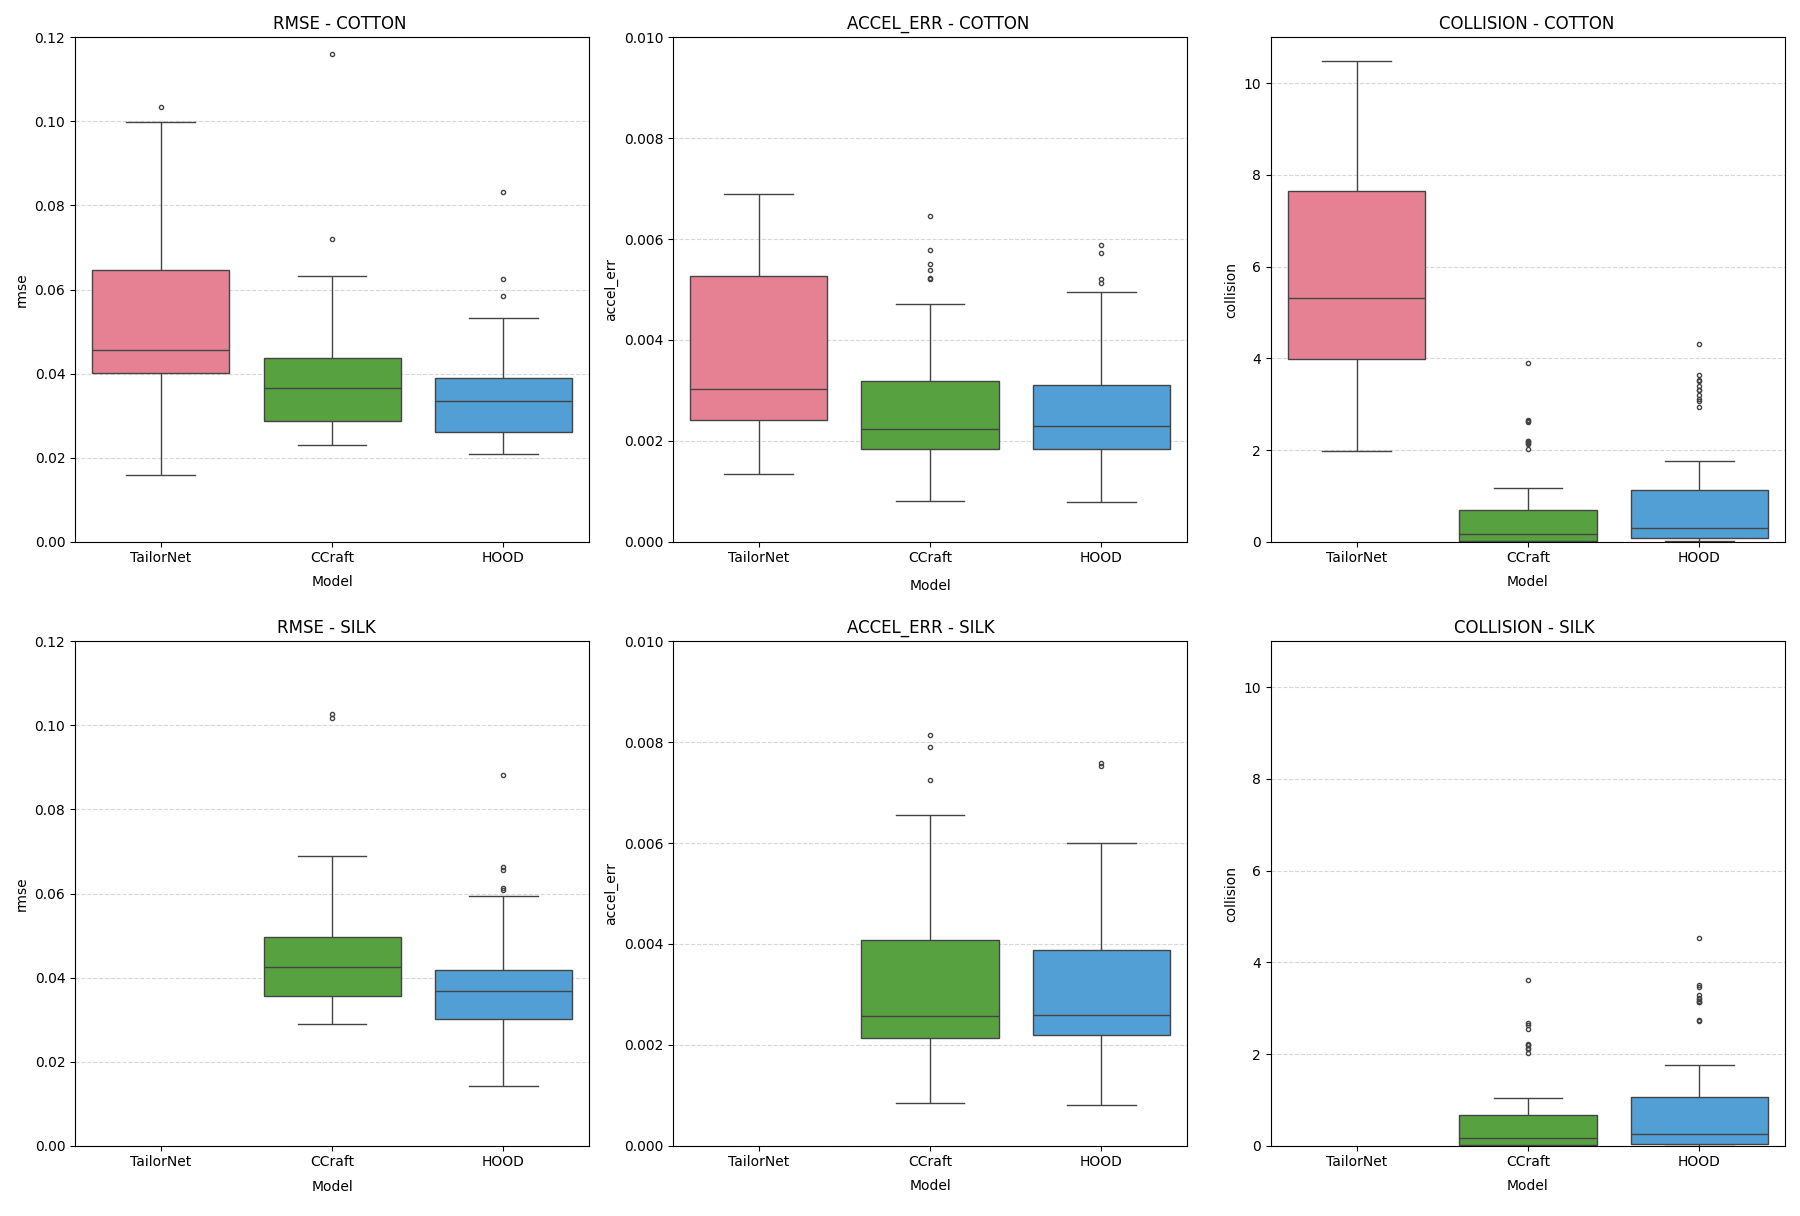
\includegraphics[width=1\textwidth]{figures/metrics_box_plots.png}
\caption{Histogrami porazdelitve metrik (RMSE, napaka pospeška in delež kolizij) čez vse testne sekvence, ločeno za bombaž in svilo.}
\label{fig:metrics_box_plots}
\end{figure}

Časovno zahtevnost smo ovrednotili z merjenjem celotnega časa izvajanja posamezne sekvence, ki smo ga nato delili s številom pripadajočih okvirjev. S tem smo pridobili povprečen čas izvajanja na okvir za vsako sekvenco posebej, te podatke pa smo nato združili v histograme za vsak model, prikazane na sliki~\ref{fig:timing_histograms}. Tukaj je vredno omeniti, da ti časi niso merili zgolj inference, ampak celotno izvajanje v okvirju, kar lahko vključuje tudi obdelavo podatkov pred in po inferenci. Ta razlika se najbolj opazi pri modelu TailorNet, saj je inferenca brez obdelave podatkov trajala povprečno le $0,08$ sekunde. Izmerjena povprečja izvajanja časovnih okvirjev pa so pokazala, da je bil model HOOD z $0,15$~s/it najučinkovitejši, sledil mu je ContourCraft z $0,64$~s/it, medtem ko je TailorNet za izračun enega okvirja potreboval $1,15$~s.

\begin{figure}[h]
\centering
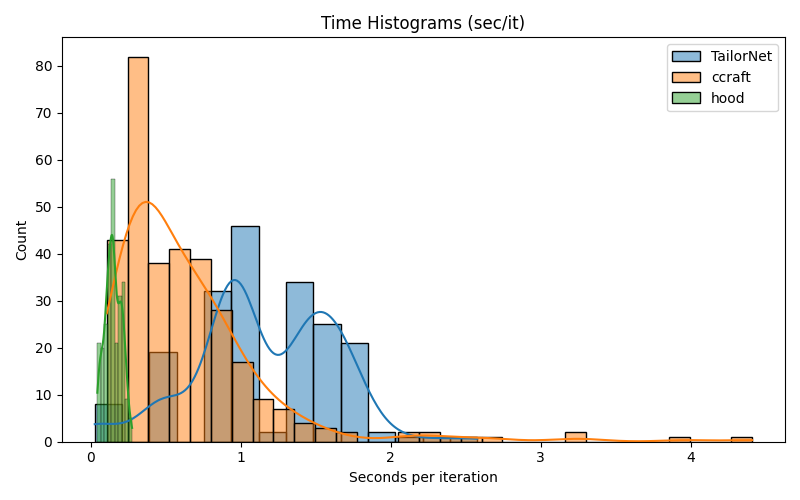
\includegraphics[width=0.8\textwidth]{figures/timing_histograms.png}
\caption{Histogrami časovne zahtevnosti inference na GPE. Prikazane so povprečne vrednosti časa na okvir za vse testne sekvence.}
\label{fig:timing_histograms}
\end{figure}

Za konec smo vizualizirali še barvne zemljevide (angl.\ \textit{heatmaps}) metrik na mreži kratke majice za en časovni okvir. Kot je prikazano na sliki~\ref{fig:error_heatmaps}, takšen prikaz omogoča neposredno identifikacijo kritičnih točk na mreži ob\-la\-či\-la. Opazili smo, da se najvišje vrednosti napak koncentrirajo v predelih rokavov, kjer so interakcije med telesom in tkanino najintenzivnejše in v sprednjem delu telesa, kjer je prisotnih največ gub.

\begin{figure}[h]
\centering
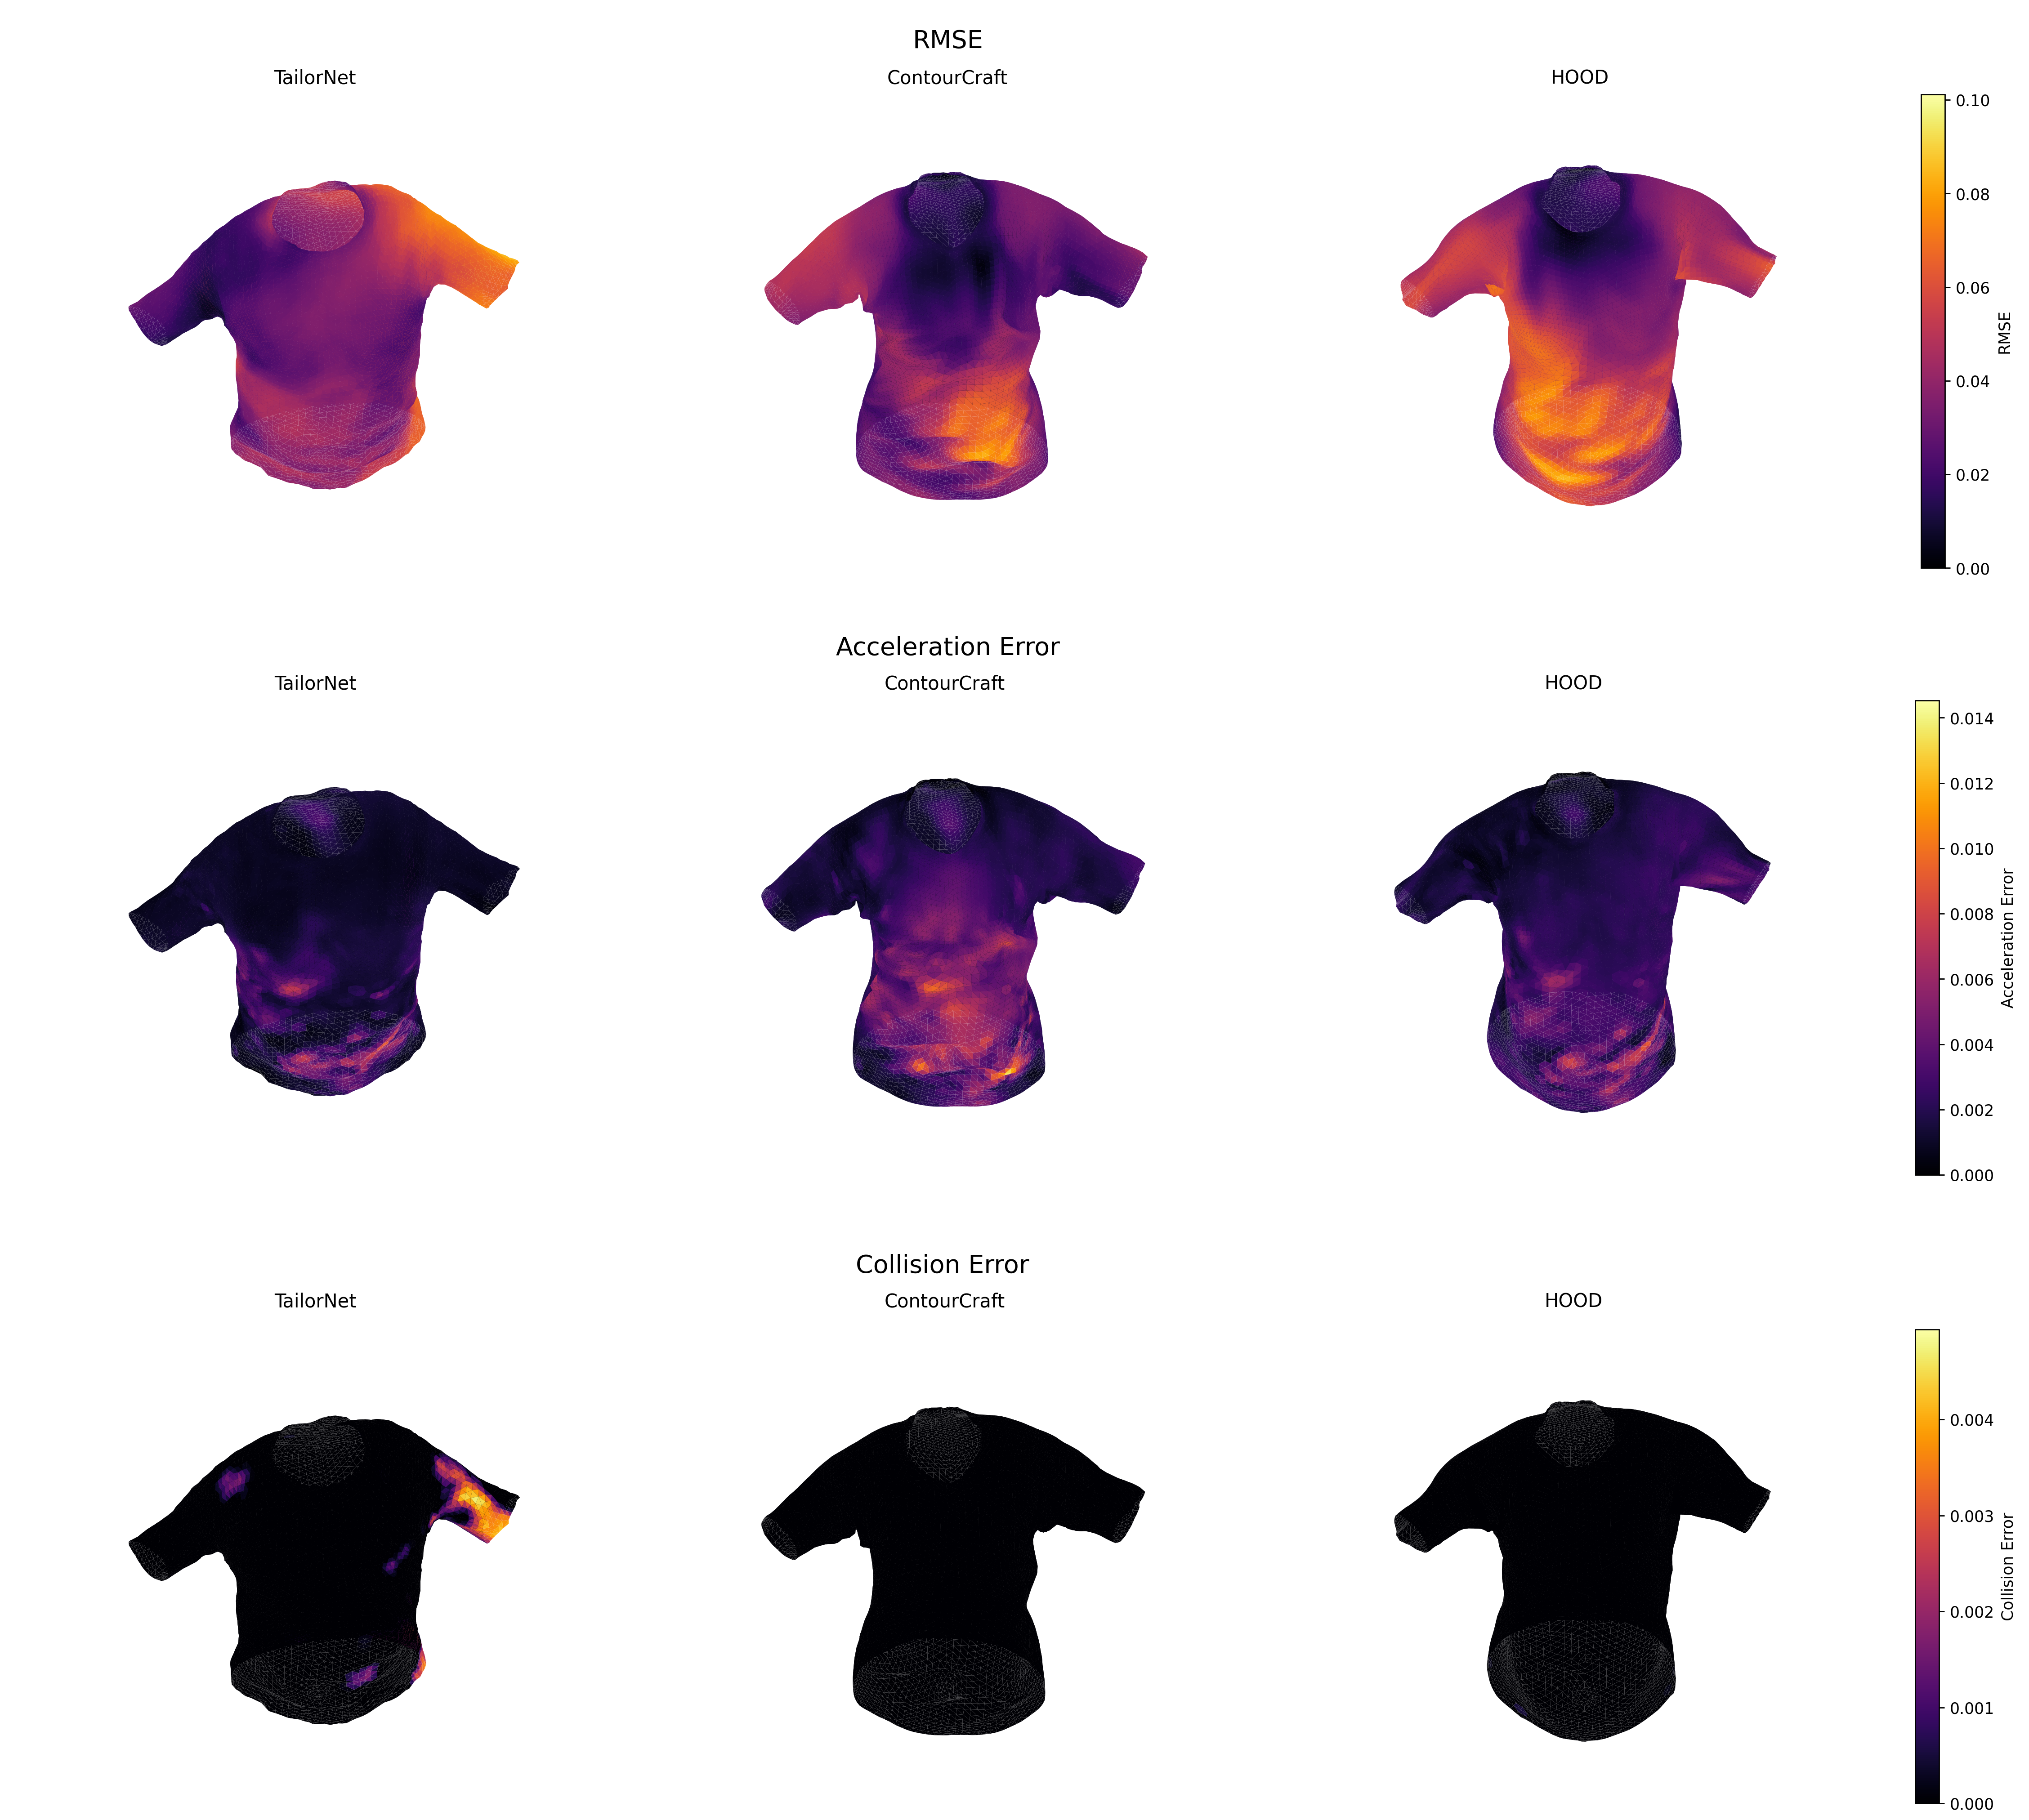
\includegraphics[width=0.9\textwidth]{figures/heatmap_results.png}
\caption{Barvni zemljevidi prostorske porazdelitve napak na modelu kratke majice. Svetla območja ponazarjajo mesta z najvišjim odstopanjem od referenčne simulacije v Mayi.}
\label{fig:error_heatmaps}
\end{figure}


\section{Izbira modela za mobilno implementacijo}
Na podlagi izvedene primerjalne analize smo za implementacijo na mobilni napravi izbrali model HOOD. Odločitev je temeljila na podlagi informacije o geometrijski natančnosti, fizikalni stabilnosti in časovni zahtevnosti inference.

Pri analizi natančnosti sta se grafna modela HOOD in ContourCraft izkazala za precej bolj robustna od modela TailorNet. HOOD je dosegel najnižji povprečni RMSE ($0,035$~m), kar predstavlja $10\,\%$ izboljšanje v primerjavi s ContourCraftom in več kot $60\,\%$ v primerjavi s TailorNetom. Čeprav je ContourCraft izkazal nekoliko večjo natančnost pri neposrednem odpravljanju kolizij, je HOOD to nadomestil z boljšo stabilnostjo pospeška, kar v praksi pomeni bolj tekočo animacijo.

Odločilni dejavnik za izbiro modela HOOD nad ContourCraftom pa je bila njegova časovna učinkovitost. S povprečnim časom $0,1490$~s na okvir je HOOD bistveno hitrejši od modela ContourCraft ($0,6432$~s). Ker mobilne naprave razpolagajo z omejenimi viri, kjer vsaka podrobnost vpliva na odzivnost sistema, HOOD nudi najboljše razmerje med vizualno kakovostjo in hitrostjo izvajanja.



%----------------------------------------------------------------
% Poglavje (Chapter) 5
%----------------------------------------------------------------
\chapter{Arhitektura modela HOOD}
\label{ch:arhitektura_modela_hood}
Za implementacijo modela HOOD~\cite{hood} na mobilnih napravah moramo podrobno poznati njegovo arhitekturo in specifične računske zahteve. V tem poglavju smo predstavili notranjo zgradbo modela, njegovo matematično osnovo ter protokol za posredovanje sporočil, kar je podlaga za kasnejše prilagoditve in optimizacijske postopke na ciljnih napravah.


\section{Zasnova sistema}
Model HOOD je zasnovan kot nevronska mreža nad grafi, ki simulira dinamiko tkanin v interakciji s kompleksnimi geometrijami, kot je človeško telo. Da vhodne podatke prilagodimo modelu, sta tridimenzionalni geometrijski mreži tkanine in telesa predstavljeni v obliki grafa, kjer oglišča mrež tvorijo vozlišča, njihovi robovi pa povezave grafa. Naloga modela je napovedati deformacijo tkanine glede na zunanje in notranje sile, kar doseže z integracijo fizikalnih principov neposredno v funkcijo izgube globokega učenja. Arhitektura je modularna, saj strogo ločuje pripravo geometrijskih podatkov od samega nevronskega računanja. Kot prikazuje slika~\ref{fig:hood_architecture}, lahko model razdelimo na: \textbf{kodirnik}, ki surove prostorske koordinate zakodira v latentni prostor, \textbf{procesor}, ki izvaja fizikalne inference z uporabo zaporednih grafnih blokov in \textbf{dekodirnik}, ki latentne predstavitve vozlišč dekodira v napovedana stanja. 
\vspace{1em}

\begin{figure}[ht]
    \centering
    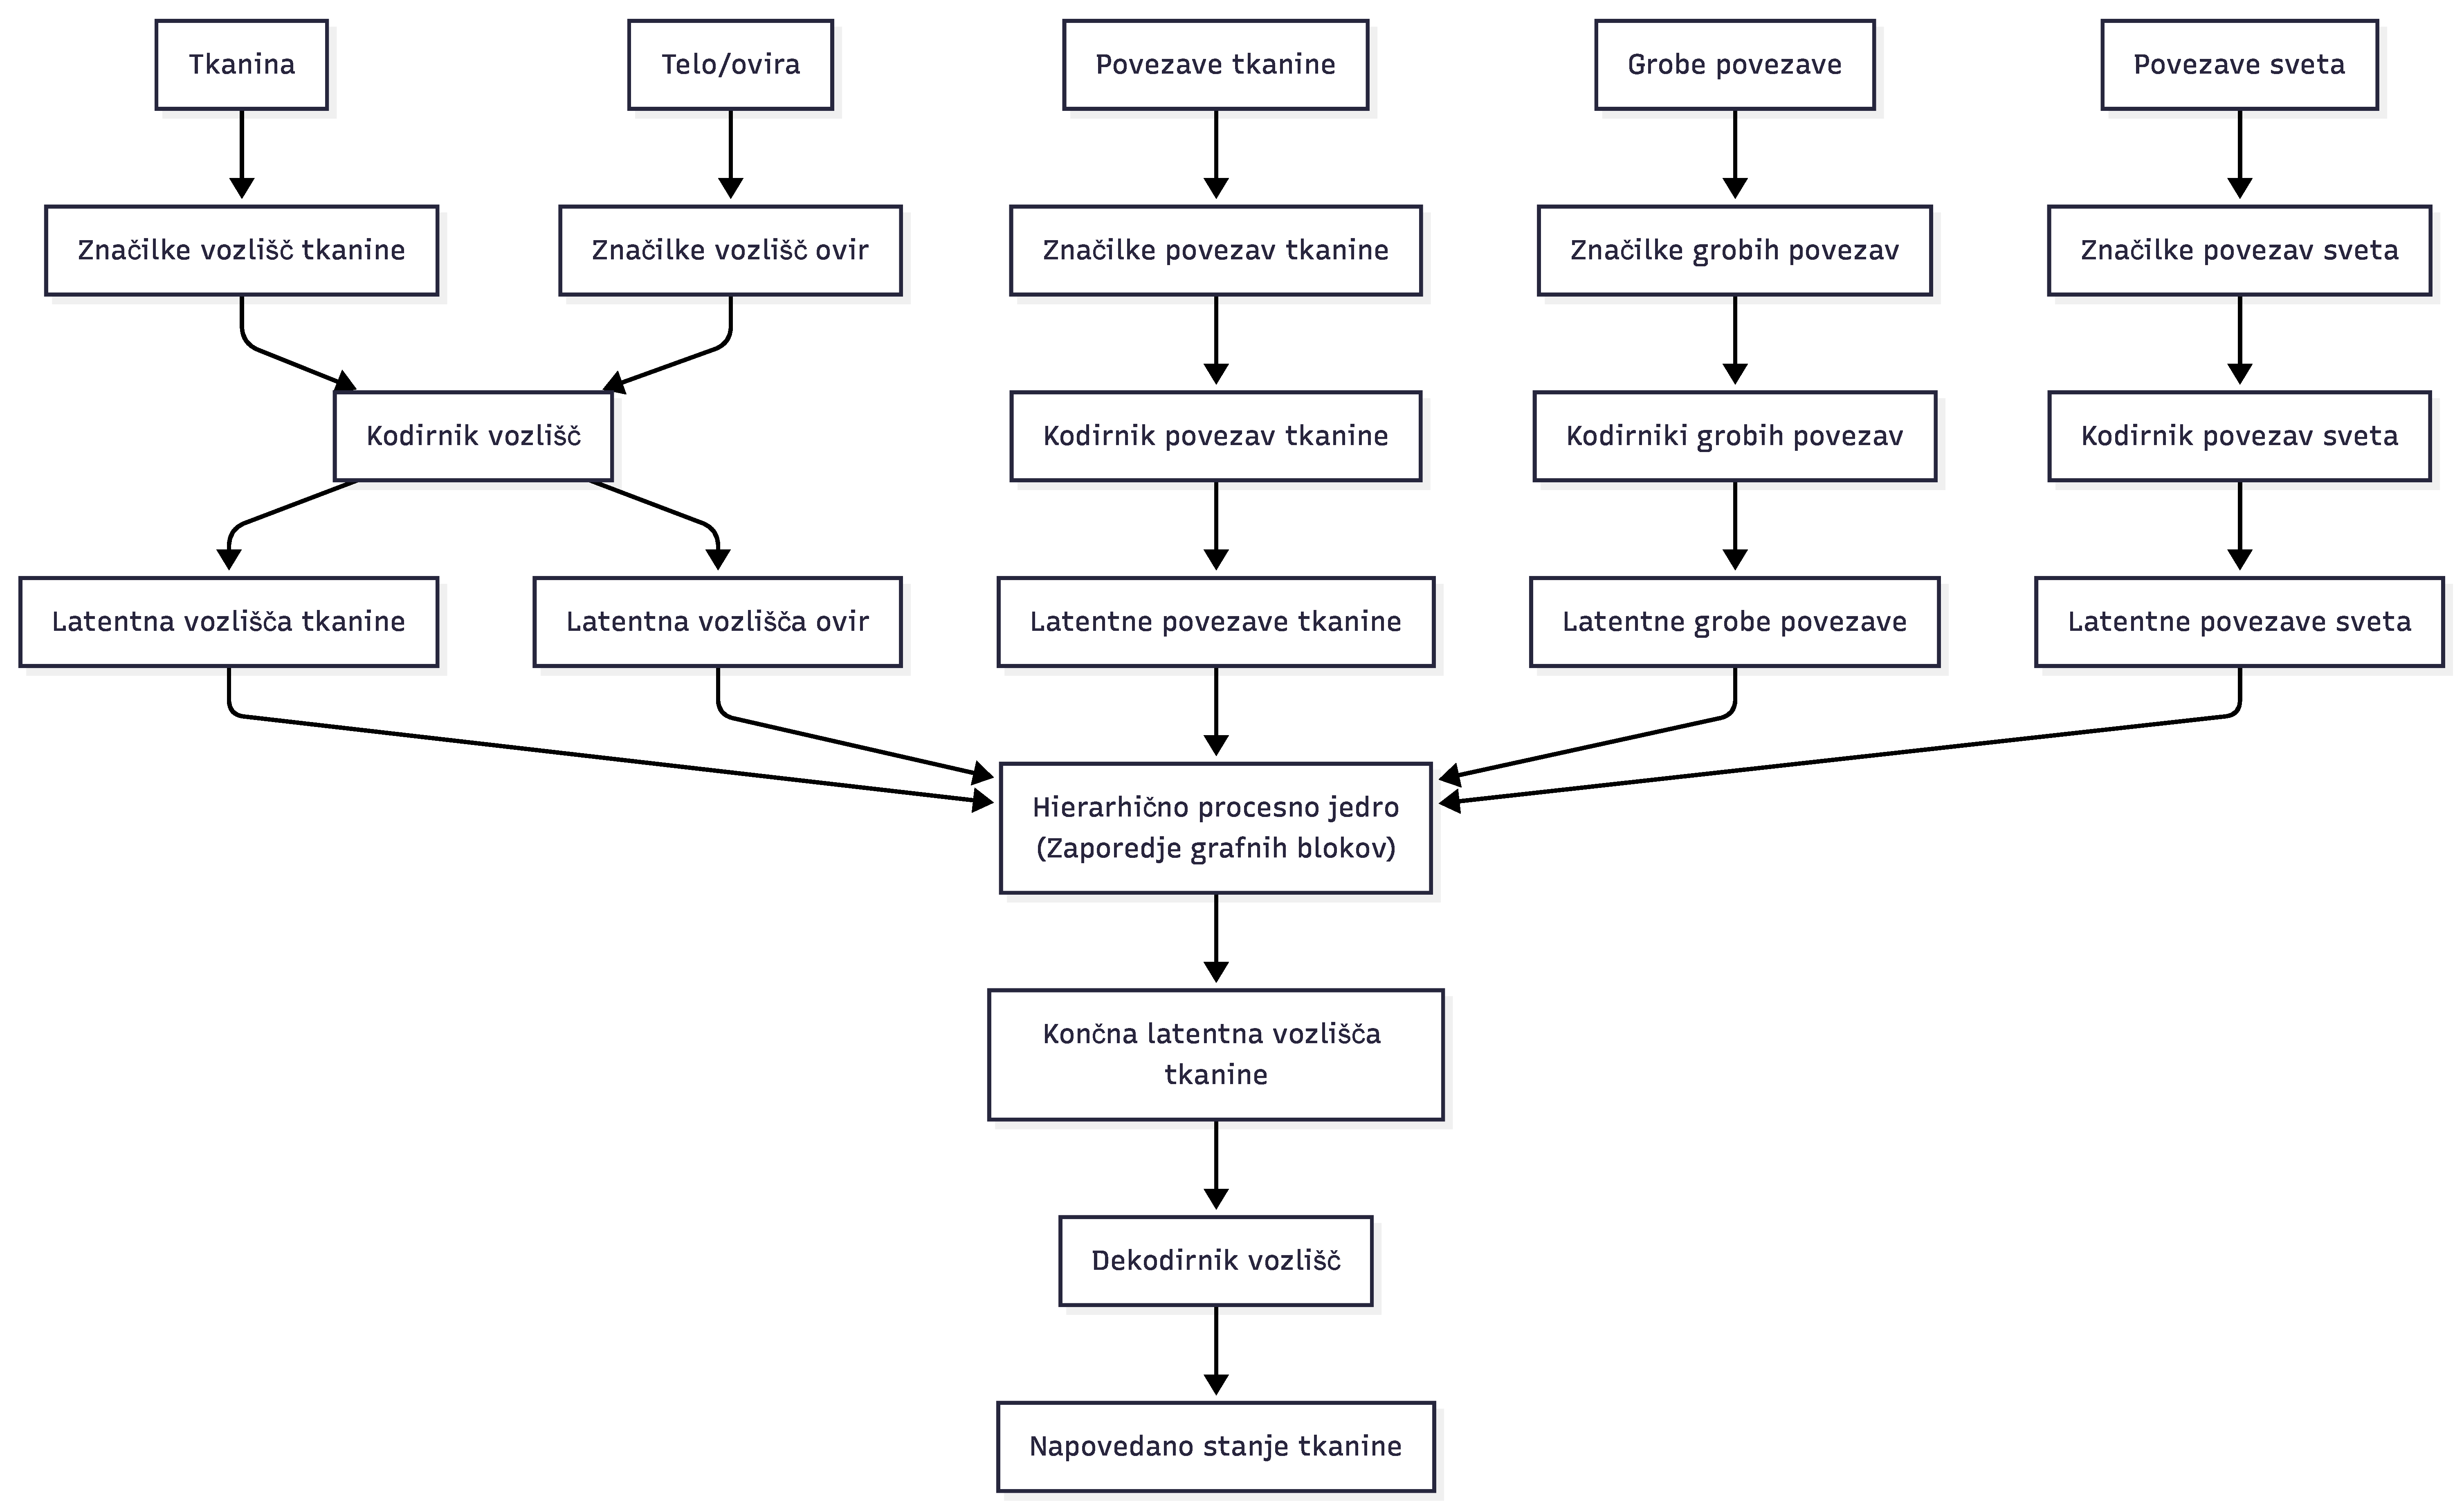
\includegraphics[width=0.95\textwidth]{figures/hood_architecture.pdf}
    \caption{Shematski prikaz arhitekture HOOD, ki temelji na principu \textit{Encode-Process-Decode}. Proces se začne z zakodiranjem vozlišč in povezav grafa tkanine in telesa, nadaljuje z latentnim procesiranjem sporočil znotraj hierarhičnega jedra in zaključi z integracijo pospeškov v nove položaje vozlišč.}
    \label{fig:hood_architecture}
\end{figure}

Proces se začne s fazo kodiranja, kjer se podatki vozlišč (položaj, hitrost, materialne lastnosti ter geometrijske povezave) preslikajo v visokodimenzionalne latentne vektorje. Računski graf v tej fazi združuje različne tipe informacij, vključno z mrežnimi povezavami tkanine, grobimi povezavami dolgega dosega ter dvosmernimi povezavami sveta, ki opisujejo interakcije med oblačilom in telesom. Za vsak tip vhodnega vektorja ima model svoj večplastni perceptron z dvema skritima plastema, ki vhodne vektorje značilk zakodira v skupni latentni prostor.

Glavni del arhitekture je hierarhično procesno jedro, ki je sestavljeno iz več zaporednih grafnih blokov. Število blokov je sicer možno prilagoditi, ampak so za model HOOD točno specificirali optimalno zaporedje. V vsakem bloku sta aktivna največ dva nivoja grobosti, ki predstavljata različne ločljivosti mreže tkanine in telesa. Znotraj posameznih blokov se s pomočjo posredovanja sporočil latentna stanja vozlišč in povezav iterativno posodabljajo. Modula za podvzorčenje in nadvzorčenje prilagajata vpliv povezav sveta glede na trenutno stopnjo hierarhije, da se lokalne in globalne deformacije širijo po celotnem grafu.

V zadnjem koraku dekodiranja se končna latentna stanja vozlišč oblačila preslikajo nazaj v tridimenzionalni fizikalni prostor. Izhod dekodirnika je trenutni pospešek vsakega posameznega vozlišča oblačila, medtem ko latentna stanja ovir v tej fazi ne sodelujejo več, saj so le notranji nosilci interakcij. Na podlagi napovedanih pospeškov se posodobijo hitrosti in položaji vozlišč tkanine za naslednji časovni korak.


\section{Hierarhična grafovska predstavitev}

\subsubsection{Definicija heterogenih vozlišč in povezav}
Model HOOD deluje nad heterogenim grafom, ki ga sestavljata dve primarni množici vozlišč: vozlišča tkanine in vozlišča ovir oziroma človeškega telesa. Vozlišča tkanine predstavljajo oglišča na mreži oblačila, vozlišča telesa pa opisujejo topologijo telesa, s katerim je oblačilo v interakciji. Prostorski odnosi med temi vozlišči so kodirani skozi več tipov povezav. Neposredna sosednost vozlišč v osnovni, fini mreži oblačila je predstavljena s povezavami mreže (\texttt{mesh\_edge}), medtem ko interakcije dolgega dosega znotraj iste tkanine opisujejo grobe povezave (\texttt{coarse\_edge0} in \texttt{coarse\_edge1}), ki omogočajo modeliranje fizikalnih sil na večje razdalje. Stik med telesom in oblačilom določajo povezave sveta (\textit{world\_edges}), ki so zaradi asimetrije med tipi vozlišč razdeljene v dve ločeni usmerjeni relaciji: neposredne povezave sveta (\texttt{world\_direct}) za posredovanje sporočil od telesa proti oblačilu ter inverzne povezave sveta (\texttt{world\_inverse}) za prenos informacij v obratni smeri.

Ker mrežne in grobe povezave povezujejo isti tip vozlišč, so znotraj posamezne množice shranjene dvosmerno, kar model doseže z avtomatskim podvajanjem povezav v obeh smereh pri pretvorbi mnogokotniške mreže. Povezave sveta pa morajo biti ločene v dve relaciji, saj se izvorni in ciljni tip vozlišča razlikujeta. Ključna arhitekturna posebnost modela HOOD je to, da grobi nivoji ne predstavljajo ločenih grafov z zmanjšanim številom vozlišč. Vsi grobi nivoji delujejo nad popolnoma enako množico vozlišč finega oblačila, spreminja pa se le nabor povezav, ki so aktivne med posredovanjem sporočil. Večnivojska obdelava v modelu HOOD zato v celoti temelji na povezavah in ne na vozliščih. To preprečuje izgubo lokalnih geometrijskih informacij med prehajanjem skozi hierarhijo.

\subsubsection{Konstrukcija povezav sveta in maskiranje}
Vhodni graf se dinamično sestavlja za vsak časovni okvir posebej znotraj pripravljalne faze modela. Najprej se fiksirana oziroma vpeta vozlišča tkanine nadomestijo z njihovimi vnaprej določenimi ciljnimi položaji, ki izhajajo iz animacije gibanja. Takoj za tem se izvede postopek za gradnjo povezav sveta na podlagi bližine med oblačilom in telesom. Za vsako vozlišče oblačila algoritem poišče bližnja vozlišča telesa, ki se nahajajo znotraj vnaprej določenega kolizijskega radija, in med njimi vzpostavi ustrezne usmerjene povezave. Pri tem so določeni deli telesa, ki so označeni kot izpuščeni (npr. določena vozlišča dlani, da se preprečijo artefakti samopresekanja), odstranjeni iz tega postopka. Ta faza iskanja sosedov hkrati ustvari tudi masko aktivnih vozlišč telesa (\texttt{active\_mask}), ki definira, katera vozlišča v trenutnem časovnem okvirju dejansko sodelujejo v interakciji z oblačilom.

Razlikovanje med aktivnimi in neaktivnimi vozlišči telesa je pomembna optimizacija modela. Aktivna vozlišča so tista, ki imajo v tekočem okvirju vzpostavljeno vsaj eno povezavo sveta z oblačilom. Neaktivna vozlišča telesa so še vedno strukturni del geometrijske mreže, vendar so popolnoma izključena iz postopka normalizacije podatkov in kasnejšega latentnega kodiranja vozlišč. Njihova latentna predstavitev se v naslednjih korakih zapolni z ničelnimi vektorji.


\section{Fizikalne in geometrijske značilke}

\subsubsection{Značilke vozlišč}
Vhodni podatki za vsako vozlišče grafa se pred vstopom v kodirnik združijo v 24-di\-men\-zio\-nal\-ni vektor surovih značilk. Ta vektor združuje kinematiko, geometrijo ter fizikalne parametre materiala in je sestavljen iz naslednjih komponent:

\begin{itemize}
\item \textbf{Trenutna hitrost vozlišča:} določa gibanje v prostoru (3 dimenzije).
\item \textbf{Vgraditev tipa vozlišča:} določa pripadnost razredu \texttt{NodeType} (9 dimenzij, čeprav se jih uporablja le 4).
\item \textbf{Vgraditev nivoja vozlišča:} označuje najgloblji nivo hierarhije, v katerem je vozlišče prisotno (4 dimenzije).
\item \textbf{Površinska normala:} opisuje lokalno orientacijo vozlišča (3 dimenzije).
\item \textbf{Časovni korak:} določa diskretni premik časa (1 dimenzija).
\item \textbf{Logaritem mase:} izhaja iz teže blaga (1 dimenzija).
\item \textbf{Koeficient upogibanja:} določa odpornost proti pregibanju (1 dimenzija).
\item \textbf{Laméjeva materialna parametra $\mu$ in $\lambda$:} določata elastične lastnosti tkanine (2 dimenziji).
\end{itemize}

Ker vozlišča ovir, ki predstavljajo človeško telo, ne uporabljajo materialnih lastnosti tkanine, so mesta za maso, koeficient upogibanja in Laméjeva parametra pri teh vozliščih nastavljena na fiksno vrednost -1.


\subsubsection{Značilke povezav}
Povezave znotraj grafa so opisane z geometrijskimi vektorji, ki omogočajo izračun sil in deformacij. Fine in grobe povezave so predstavljene z 12-dimenzionalnim vektorjem značilk, ki ga sestavljajo naslednje komponente:

\begin{itemize}
\item \textbf{Trenutni relativni položaj:} določa trenutni odmik med povezanima vozliščema (3 dimenzije).
\item \textbf{Trenutna razdalja:} določa trenutno evklidsko razdaljo med voz\-li\-ščema (1 dimenzija).
\item \textbf{Relativni položaj v mirovanju:} določa relativni položaj vozlišč v nevtralnem stanju tkanine (3 dimenzije).
\item \textbf{Razdalja v mirovanju:} določa razdaljo med vozliščema v nevtralnem stanju tkanine (1 dimenzija).
\item \textbf{Časovni korak:} določa diskretni premik časa (1 dimenzija).
\item \textbf{Materialni parametri:} vključujejo Laméjeva parametra $\mu$ in $\lambda$ ter koeficient upogibanja (3 dimenzije).
\end{itemize}

Ti podatki modelu omogočajo primerjavo trenutne geometrije z začetnim stanjem, kar je podlaga za modeliranje natega, stiskanja in upogiba tkanine.

Povezave sveta uporabljajo 9-dimenzionalni vektor značilk, ki opisuje trenutno in prihodnjo geometrijo stika med tkanino in telesom:

\begin{itemize}
\item \textbf{Trenutni relativni odmik:} določa trenutni odmik med vozliščem oblačila in vozliščem telesa (3 dimenzije).
\item \textbf{Trenutna razdalja:} določa trenutno evklidsko razdaljo med njima (1 dimenzija).
\item \textbf{Prihodnji relativni odmik:} določa odmik do položaja telesa v naslednjem ča\-sov\-nem koraku (3 dimenzije).
\item \textbf{Prihodnja razdalja:} določa razdaljo v naslednjem koraku (1 dimenzija).
\item \textbf{Časovni korak:} določa diskretni premik časa (1 dimenzija).
\end{itemize}

Pri inverznih povezavah sveta se smerni odmiki negirajo, s čimer se ohrani pravilna orientacija prostorskih vektorjev.


\section{Latentno kodiranje in grafni blok}
\label{sec:latentno_kodiranje_in_grafni_blok}
Faza preslikave izvornih značilk v latentni prostor poteka ločeno za vozlišča in povezave z uporabo namenskih kodirnikov, ki — tako kot vsi preostali nevronski moduli v arhitekturi HOOD — temeljijo na večplastnih perceptronih z dvema skritima plastema velikosti $128$. Pri kodiranju vozlišč si tkanina in telo delita skupni kodirnik (\texttt{node\_encoder}). Zaradi računske učinkovitosti se vektorji značilk združijo v matriko vzdolž dimenzije števila vozlišč, nad katero se s kodirnikom izvede transformacija. Po končanem prehodu se dobljeni latentni tenzor razporedi nazaj na ločeni stanji oblačila in telesa, medtem ko se neaktivna vozlišča telesa zapolnijo z ničelnimi vektorji. Pri povezavah model uporablja svoj kodirnik za vsak tip povezave posebej, pri čemer si neposredne in inverzne povezave sveta delijo skupni kodirnik povezav sveta. HOOD tako vključuje štiri kodirnike za povezave: \texttt{mesh\_edge\_encoder}, \texttt{coarse\_edge0\_encoder}, \texttt{coarse\_edge1\_encoder} in \texttt{wo\-rld\_edge\_encoder}.

Ko so začetna latentna stanja pripravljena, vstopijo v hierarhično procesno jedro, ki je sestavljeno iz grafnih blokov, imenovanih \texttt{GraphNetBlocks}. Ti bloki si sledijo v zaporedju, vsak pa ima aktivirane le določene tipe povezav, da se informacija o deformacijah postopoma prenaša med različnimi prostorskimi ločljivostmi, kar podrobno opišemo v poglavju~\ref{sec:vecnivojsko_posredovanje_sporočil}. Da pa lahko razumemo pretok informacij skozi celotno jedro, najprej natančno analiziramo notranjo zgradbo posameznega grafnega bloka. Tok podatkov znotraj ene takšne računske enote prikazuje slika~\ref{fig:graph_net_block}.

\begin{figure}[ht]
\centering
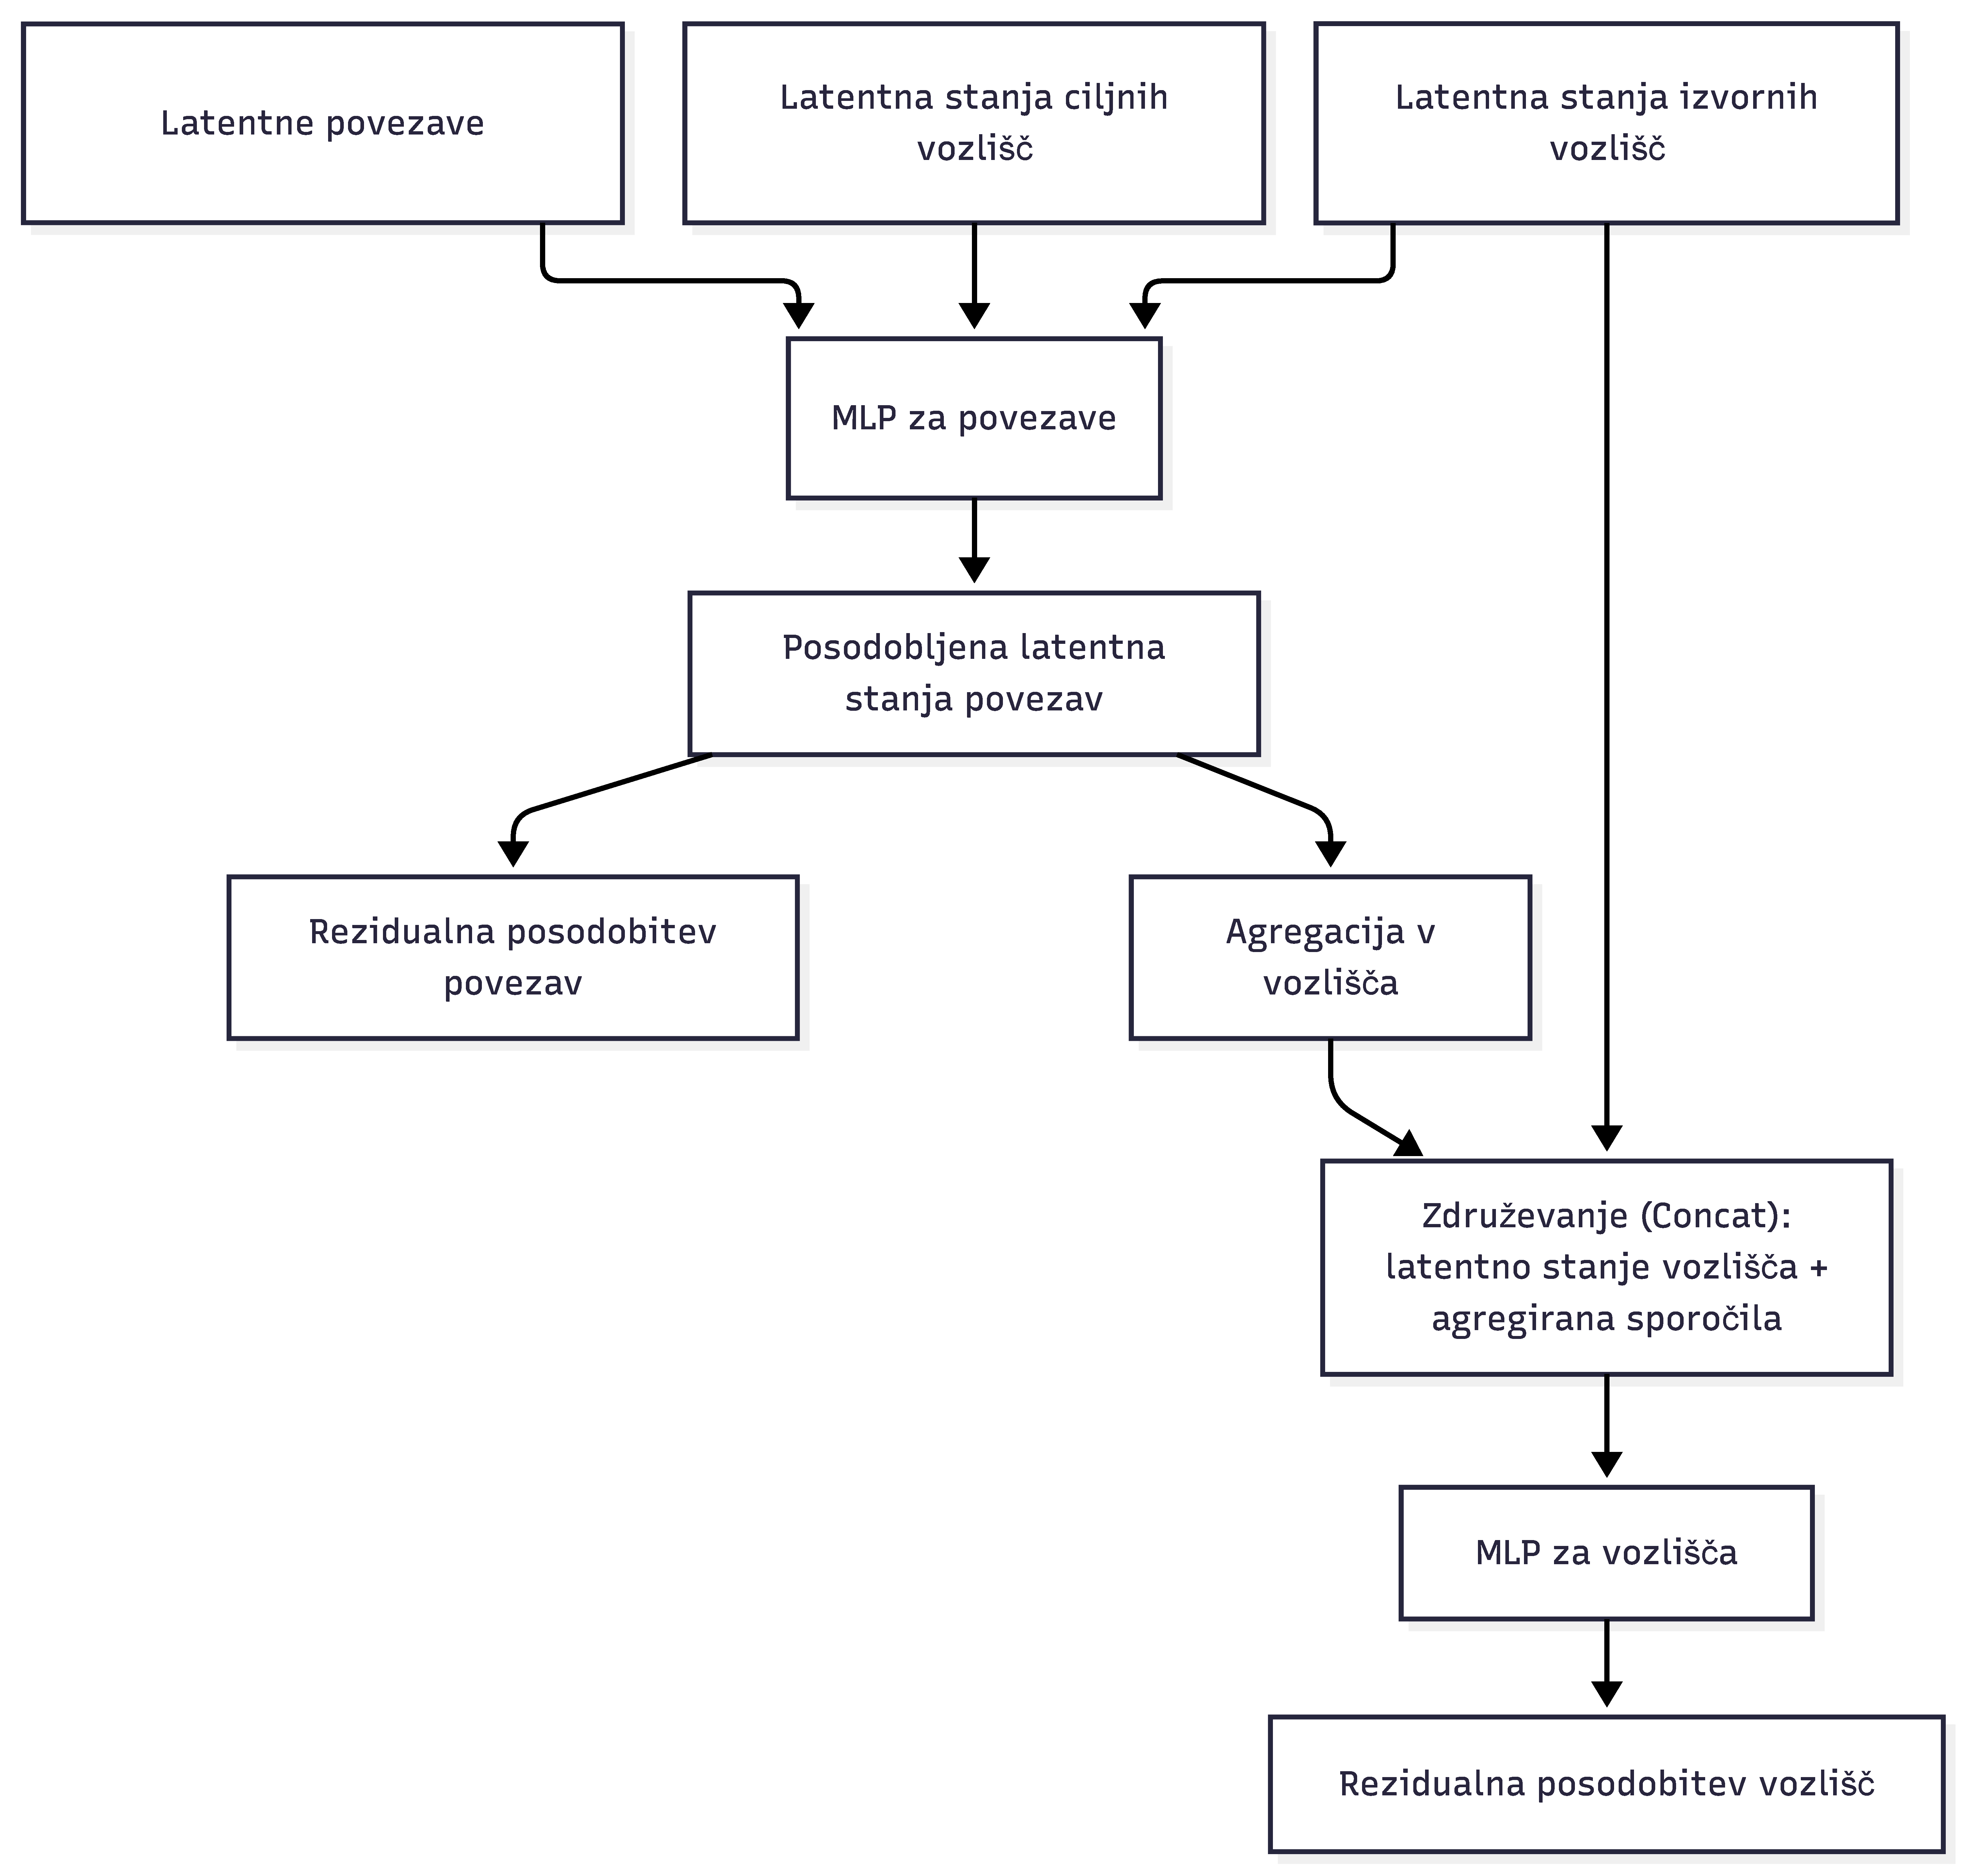
\includegraphics[width=0.9\textwidth]{figures/graph_net_block.pdf}
\caption{Diagram operacij znotraj enega grafnega bloka. Prikazan je mehanizem posodobitve povezav, agregacije s funkcijo scatter-sum in končne rezidualne posodobitve latentnih stanj.}
\label{fig:graph_net_block}
\end{figure}

Znotraj vsakega bloka se najprej posodobijo latentna stanja vseh aktivnih povezav. Za vsako usmerjeno povezavo model združi trenutno latentno stanje ciljnega vozlišča, izvornega vozlišča in same povezave v en vektor. Ta vektor potuje skozi MLP za povezave, kar formalno opišemo z enačbo:
$$\Delta e_{ij} = \phi_e([h_j, h_i, e_{ij}]),$$
kjer $i$ predstavlja izvorno vozlišče, $j$ ciljno vozlišče, $e_{ij}$ trenutno stanje povezave, $\phi_e$ večplastni perceptron za povezave, $\Delta e_{ij}$ pa izračunana delta značilk povezave. Ti vektorji delta značilk povezav se nato preko operacije sumacije (\texttt{scatter\_sum}) agregirajo v ciljna vozlišča. Model to agregacijo izvaja ločeno glede na tip povezave. Posamezno vozlišče tkanine tako prejme ločene agregirane vektorje iz povezav sveta, mrežnih povezav in vsakega aktivnega grobega nivoja posebej:
$$a_j^r = \sum_{i \in \mathcal{N}_r(j)} \Delta e_{ij}^r,$$
kjer je $r$ tip povezave, $\Delta e_{ij}^r$ izračunana delta značilk povezave, ki se uporabi kot sporočilo, $a_j^r$ pa agregiran vektor sporočil povezav tipa $r$. Končni korak znotraj bloka predstavlja posodobitev latentnih stanj vozlišč. Vsi ločeno agregirani vektorji sporočil se združijo s trenutnim latentnim stanjem vozlišča in gredo skozi MLP za vozlišča:
$$\Delta h_j = \phi_v([h_j, a_j^{\text{world}}, a_j^{\text{mesh}}, a_j^{\text{coarse0}}, a_j^{\text{coarse1}}]),$$
kjer $a_j$ predstavlja agregirana sporočila posameznega tipa povezave, $h_j$ trenutno latentno stanje vozlišča, $\phi_v$ pa MLP za vozlišča.

Ključna lastnost grafnega bloka je rezidualna zasnova. Model obstoječih stanj ne nadomesti neposredno z novimi izračuni, temveč napove delte in jih prišteje k trenutni vrednosti:
$$e^{t+1} = e^t + \Delta e^t,$$
$$h^{t+1} = h^t + \Delta h^t.$$

V smeri posredovanja sporočil povezave mreže in grobe povezave pre\-na\-šajo informacije dvosmerno med vozlišči tkanine, neposredne povezave sveta pre\-na\-šajo vpliv telesa na oblačilo, inverzne povezave sveta pa omogočajo, da informacije o stanju tkanine vplivajo nazaj na latentno stanje telesa.


\section{Večnivojsko posredovanje sporočil}
\label{sec:vecnivojsko_posredovanje_sporočil}

\subsubsection{Komunikacija nivojev}
Hierarhična struktura modela HOOD ne temelji na krčenju ali združevanju vozlišč v manjše grafe, temveč na hkratnem obstoju več ravni grobosti nad isto množico vozlišč tkanine. Prehod informacij med finimi mrežnimi povezavami (\texttt{mesh\_edge}) in grobimi povezavami dolgega dosega (\texttt{coarse\_edge}) poteka neposredno prek deljenega latentnega stanja vozlišč $h$. Ko se izvede grafni blok, ki uporablja fine povezave, se posodobijo latentni vektorji vozlišč na podlagi lokalne topologije. Ko naslednji grafni blok aktivira grobe povezave, ti isti latentni vektorji vozlišč sprejmejo informacije iz večjih prostorskih razdalj. Latentni tenzor vozlišč tkanine tako deluje kot osrednje komunikacijsko križišče, skozi katerega se informacije iz različnih prostorskih ločljivosti zlivajo in izmenjujejo brez potrebe po eksplicitnih povezavah med finimi in grobimi vozlišči.

\subsubsection{Hierarhično procesno jedro}
Hierarhično procesno jedro modela sestavlja zaporedje petnajstih grafnih blokov, ki so razdeljeni v pet faz:

\begin{itemize}
\item \textbf{Prva faza} vsebuje prve tri bloke. V njih se aktivirajo tri vrste povezav: mrežne povezave \texttt{mesh\_edge}, povezave prvega nivoja grobosti \texttt{coarse\_edge0} in povezave sveta. V prvi fazi model hkrati obdeluje lokalne sile tkanine in interakcije daljšega dosega.
\item \textbf{Druga faza} se začne z modulom za podvzorčenje \texttt{DownSample}, ki se izvede pred prvim grafnim blokom druge faze. Ta modul ne zmanjša števila vozlišč, temveč iz grafa odstrani povezave sveta, ki niso povezane z vozlišči, vključenimi v višje nivoje hierarhije. V vseh treh blokih druge faze model izklopi mrežne povezave in upošteva le povezave prvega in drugega nivoja grobosti (\texttt{coarse\_edge0} in \texttt{coarse\_edge1}) ter povezave sveta. Z izklopom mrežnih povezav model usmeri računsko moč v širjenje globalnih upogibov in gub daljšega dosega.
\item \textbf{Tretja faza} v modulu za podvzorčenje izključi povezave prvega nivoja grobosti (\texttt{coarse\_edge0}). Sledi procesiranje v treh grafnih blokih, kjer ostanejo aktivne le grobe povezave drugega nivoja (\texttt{coarse\_edge1}) in povezave sveta. To je najgloblji del hierarhije, kjer model procesira globalne topološke lastnosti tkanine in premike telesa.
\item \textbf{Četrta faza} vsebuje modul za nadvzorčenje \texttt{UpSample}, ki ponovno vključi povezave prvega nivoja grobosti (\texttt{coarse\_edge0}) in povezave sveta, ki so povezane s trenutno aktivnimi vozlišči. V vseh treh blokih četrte faze so torej upoštevane povezave \texttt{coarse\_edge0}, \texttt{coarse\_edge1} in povezave sveta, kar omogoči prenos informacij iz globalnega prostora nazaj proti lokalni ravni.
\item \textbf{Peta faza} vsebuje zadnje tri zaporedne grafne bloke. Pred začetkom pete faze modul za nadvzorčenje v graf vrne predhodno odstranjene povezave sveta in fine mrežne povezave (\texttt{mesh\_edge}), aktivne pa ostanejo tudi povezave prvega nivoja grobosti (\texttt{coarse\_edge0}). V peti fazi model pridobljene globalne informacije ponovno uskladi z lokalnimi geometrijskimi detajli fine mreže.
\end{itemize}

Opisani cevovod zagotavlja razporeditev informacij o trkih in premikih telesa po celotni strukturi tkanine. V vsakem bloku so hkrati aktivni največ trije tipi relacij, kar omejuje računsko zahtevnost.


\section{Dekodiranje in integracija pospeškov}
Po zaključku procesne faze model končna latentna stanja vozlišč tkanine preslika nazaj v tridimenzionalni fizikalni prostor. Dekodiranje izvedemo z namenskim dekodirnikom vozlišč (\texttt{node\_decoder}), ki temelji na večplastnem perceptronu z dvema skritima plastema. Dekodirnik sprejme končne visokodimenzionalne latentne vektorje vozlišč tkanine $h^{\text{cloth}}$, medtem ko latentna stanja vozlišč telesa v fazi dekodiranja ne sodelujejo več, saj so služila le kot notranji nosilci interakcij med posredovanjem sporočil. Izhod dekodirnika je trenutni pospešek vsakega posameznega oglišča 3D-mreže oblačila:
$$a_t = \phi_d\left(h_t^{\text{cloth}}\right),$$
kjer $a_t$ predstavlja vektor tridimenzionalnega pospeška v trenutnem ča\-sov\-nem okviru $t$, $\phi_d$ označuje večplastni perceptron dekodirnika, $h_t^{\text{cloth}}$ pa predstavlja latentno stanje vozlišča tkanine.

Na podlagi napovedanih pospeškov in časovnega koraka model izračuna novo hitrost oglišč mreže oblačila:
$$v_{t+1} = v_t + a_t \cdot \Delta t,$$
kjer $v_t$ označuje trenutno hitrost oglišča, $v_{t+1}$ posodobljeno hitrost za naslednji časovni korak, $\Delta t$ pa diskretni časovni korak simulacije. Takoj po izračunu novih hitrosti se posodobijo še prostorski položaji oglišč oblačila:
$$x_{t+1} = x_t + v_{t+1} \cdot \Delta t,$$
kjer $x_t$ predstavlja trenutne koordinate oglišča, $x_{t+1}$ pa nov izračunan položaj.

Zadnji korak je uveljavitev robnih pogojev in vnaprej določenega premikanja telesa. Upoštevati moramo definirana vpeta oglišča oblačila, kot so deli okoli pasu ali ovratnika, ki sledijo gibanju človeškega telesa. Z uporabo binarne maske za vsa vpeta oglišča model zavrže napovedane položaje $x_{t+1}$ in jih prepiše z določenimi ciljnimi položaji, izračunanimi z algoritmom za oblačenje na podlagi skeletne animacije telesa. Z opisanim postopkom zagotovimo, da oblačilo natančno sledi ključnim opornim točkam animacije, preostali prosti deli tkanine pa se dinamično odzivajo na simulirane sile.



%----------------------------------------------------------------
% Poglavje (Chapter) 6
%----------------------------------------------------------------
\chapter{Mobilna implementacija modela HOOD}
\label{ch:mobilna_implementacija_modela_hood}
Prenos inferenčnega cevovoda modela HOOD~\cite{hood} na operacijski sistem Android je zapleten, saj domorodna mobilna okolja ne podpirajo neposredno vseh plasti grafnih nevronskih mrež ter fizikalnih integratorjev. Razvoj smo zastavili kot iterativni proces, v katerem na enakih vhodnih podatkih preizkusimo in primerjamo več različnih mobilnih ogrodij ter strojnih po\-spe\-še\-val\-ni\-kov. Cilj takšne zasnove je stroga ločitev čistega časa izvajanja nevronskih mrež od sistemskih stroškov operacijskega sistema. Ker so posamezne strojno pospešene poti med poskusi povzročale numerični odmik ali pa so nenačrtovano preklopile nazaj na procesorsko izvajanje, poleg hitrosti merimo tudi numerično natančnost posameznih particij modela.

V nadaljevanju poglavja opisujemo iterativni potek implementacije, kjer ugotovitve in omejitve vsake faze utemeljujejo prehod na naslednje nizkonivojske tehnologije.


\section{Vzpostavitev referenčne poti}
Namesto izvajanja celotne geometrijske predobdelave na napravi smo pripravljene okvire realnih sekvenc izvozili v binarne datoteke znotraj sredstev aplikacije, saj smo bili osredotočeni na evalvacijo nevronske mreže, ki je glavni del računske obremenitve. Vsak izvoženi okvir vsebuje podatke o geometriji oblačila, geometriji človeškega telesa ter pri\-ča\-ko\-va\-nih izhodih za validacijo. Da bi se izognili masivnemu podvajanju shranjenih vmesnih tenzorjev in aplikacijo približali realnemu produkcijskemu okolju, celoten nabor izvornih značilk rekonstruiramo lokalno na napravi iz teh nizkonivojskih podatkov. Aplikacija na napravi samodejno izračunava površinske normale, določa dinamične povezave sveta znotraj kolizijskega radija ter izvaja filtriranje vozlišč z aktivno masko telesa. Pred vstopom v kodirnik vozlišč program izvede konkatenacijo vozlišč tkanine izključno z aktivnimi vozlišči telesa.

Za preverjanje pravilnosti izvajanja smo implementirali sprotno validacijo preko preverjanja največje absolutne razlike med vrednostmi namiznega cevovoda in vrednostmi mobilne aplikacije. Pri tem posamezen primerjani vmesni rezultat obravnavamo kot vektor $v$. Največjo absolutno razliko označimo z $d_{\max}$ in jo izračunamo kot:
$$d_{\max} = \max_i \left| v^{\mathrm{mobile}}_i - v^{\mathrm{expected}}_i \right|,$$
kjer je $v^{\mathrm{mobile}}$ vektor vrednosti, izračunanih v mobilni aplikaciji, $v^{\mathrm{expected}}$ vektor pri\-ča\-ko\-va\-nih vrednosti, izvoženih iz namiznega cevovoda, $i$ pa indeks posameznega elementa vektorja. Z uveljavitvijo tega mehanizma aplikacija sproti preverja vmesne rezultate, kot so izračunane vhodne značilke, izhodi kodirnikov, agregirani vektorji pri posredovanju sporočil in posodobitve znotraj grafnega bloka, ter jih primerja s pričakovanimi binarnimi vrednostmi, izvoženimi iz namiznega cevovoda.

Za izhodišče za ocenjevanje stabilnosti, pravilnosti in hitrosti smo vzpostavili referenčno pot z uradnim ogrodjem ONNX Runtime (ORT)\footnote{\url{https://onnxruntime.ai/}} na centralni procesni enoti (CPE). Neposreden izvoz celotnega modela HOOD v enoten graf ONNX ni bil izvedljiv, saj model uporablja dinamično logiko heterogenih grafov, ki temelji na strukturah \texttt{torch\_geometric.HeteroData}. Poleg tega zgodnje izvozne različice ONNX niso podpirale vseh potrebnih operatorjev, na primer plastne normalizacije -- \texttt{LayerNorm}. Zato smo model razdelili na več manjših particij ONNX, kot so kodirniki vozlišč, kodirniki povezav ter izbrane MLP particije znotraj blokov grafne nevronske mreže. Dinamično grafno logiko, pripravo povezav, agregacijo in posredovanje sporočil smo nato implementirali neposredno v mobilni aplikaciji. Ker knjižnica \texttt{onnxruntime-android} ne podpira operacije \texttt{scatter\_sum}, uporabljene v grafnih blokih, smo ročno implementirali še algoritem po\-šil\-jan\-ja sporočil v komponenti \texttt{CpuScatterSum.kt}. V kasnejših poskusih z razdeljenimi particijami ONNX smo na procesorju CPE ročno izvedli tudi \texttt{LayerNorm}, saj so bili nekateri strojno pospešeni ponudniki izvajanja primerni le za telesa perceptronov MLP, ne pa za celotno zaporedje \texttt{MLP + LayerNorm}.

Izvajanje modela smo preizkusili na več mobilnih napravah, za referenčno platformo pa smo vzeli napravo OnePlus Nord CE 3 Lite. Statistične analize povprečnih časov in standardnih odklonov za vse faze testiranja modela smo izračunali na podlagi 20 zaporednih meritev, rezultati pa so predstavljeni v tabeli~\ref{tab:cpu_detailed_breakdown}.


\begin{table}[ht!]
\centering
\caption{Povprečni časi izvajanja in statistični odkloni posameznih faz znotraj referenčne poti ORT CPE pri 20 ponovitvah.}
\label{tab:cpu_detailed_breakdown}
\begin{tabular}{lcc}
\hline
\textbf{Merjena faza cevovoda} & \textbf{Povprečni čas (ms)} & \textbf{StdDev (ms)} \\
\hline
Priprava vhodnih podatkov & $5644{,}28$ & $1977{,}64$ \\
MLP za povezave fine mreže & $2307{,}19$ & $238{,}95$ \\
MLP za povezave nivoja 0 & $2143{,}33$ & $240{,}67$ \\
MLP za povezave nivoja 1 & $1089{,}59$ & $214{,}39$ \\
MLP za povezave sveta & $1381{,}14$ & $230{,}99$ \\
MLP za vozlišča & $1553{,}25$ & $218{,}36$ \\
Ustvarjanje seje grafnih blokov & $695{,}94$ & $180{,}82$ \\
Agregacija za povezave fine mreže & $122{,}97$ & $32{,}16$ \\
Agregacija za povezave nivoja 0 & $114{,}17$ & $13{,}07$ \\
Agregacija za povezave nivoja 1 & $64{,}99$ & $3{,}44$ \\
Agregacija za povezave sveta & $156{,}30$ & $34{,}96$ \\
Kodirnik povezav fine mreže & $180{,}38$ & $60{,}11$ \\
Kodirnik povezav nivoja 0 & $98{,}32$ & $32{,}04$ \\
Kodirnik povezav nivoja 1 & $67{,}47$ & $22{,}97$ \\
Kodirnik povezav sveta & $70{,}29$ & $30{,}44$ \\
Kodirnik vozlišč & $83{,}90$ & $18{,}72$ \\
Faza podvzorčenja (\texttt{DownSample}) & $38{,}16$ & $12{,}77$ \\
Faza nadvzorčenja (\texttt{UpSample}) & $18{,}30$ & $3{,}44$ \\
Dekodirnik vozlišč & $22{,}42$ & $5{,}93$ \\
% Komentirani časi so že vključeni v meritev 'Priprava vhodnih podatkov'
% Iskanje povezav sveta & $4205{,}55$ & $2145{,}83$ \\
% Priprava mrežnih povezav & $120{,}23$ & $106{,}56$ \\
% Priprava normal človeškega telesa & $92{,}10$ & $49{,}43$ \\
% Priprava normal tkanine & $65{,}61$ & $51{,}49$ \\
% Priprava vozlišč tkanine & $71{,}00$ & $48{,}60$ \\
% Priprava neposrednih povezav sveta & $52{,}48$ & $43{,}23$ \\
% Priprava inverznih povezav sveta & $56{,}32$ & $52{,}55$ \\
% Priprava grobih povezav nivoja 0 & $33{,}47$ & $21{,}89$ \\
% Priprava grobih povezav nivoja 1 & $26{,}62$ & $16{,}97$ \\
% Priprava grobih povezav nivoja 2 & $16{,}34$ & $9{,}86$ \\
% Priprava vozlišč človeškega telesa & $11{,}10$ & $9{,}04$ \\
\hline
\textbf{Celoten okvir} & $\mathbf{15852{,}41}$ & $\mathbf{3287{,}01}$ \\
\hline
\end{tabular}
\end{table}

Analiza podatkov kaže, da skupni povprečni čas obdelave okvira znaša $15,9\text{ s}$ s standardnim odklonom $3{,}29\text{ s}$. Največ časa vzame izvajanje komponent MLP, saj vsota njihovih časov izvajanja znaša $8{,}48\text{ s}$.

Da bi ocenili vpliv same zmogljivosti procesorja na časovno zahtevnost dinamičnih faz, smo enak cevovod ORT CPE brez strojnega pospeševanja preizkusili še na najnovejši napravi Samsung Galaxy S26+. Rezultati te meritve kažejo skok v računski moči, saj je skupni čas obdelave okvira padel na $2{,}66\text{ s}$.

Glavni razlog za skoraj 6-kratno pohitritev v primerjavi z referenčno napravo OnePlus je hitrejše izvajanje faze priprave vhodnih podatkov, ki se je na napravi Samsung skrajšala na $453{,}52\text{ ms}$. Ti podatki potrjujejo, da sodobna visoko zmogljiva procesorska jedra z naprednejšim upravljanjem predpomnilnika uspešno zmanjšujejo časovni vpliv dinamičnih operacij nad grafi. To spoznanje služi kot indikator, da lahko že sam naraven razvoj mobilnih procesorjev znatno približa fizikalne simulacije izvajanju v realnem času. Ker osrednji CPE cevovod ohranja popolno numerično natančnost z odstopanjem pod $10^{-6}$, predstavlja zanesljivo izhodišče za naslednji korak, kjer poskušamo težke linearne plasti prenesti na strojne pospeševalnike. V nadaljevanju bomo zaradi preglednosti predstavili zgolj meritve na napravi OnePlus.


\section{Ponudnika izvajanja NNAPI ter XNNPACK}
Zaradi visoke časovne zahtevnosti osnovnega cevovoda smo v naslednjem koraku poskusili aktivirati strojno pospeševanje na mobilni napravi. Za ta namen smo celotno arhitekturo HOOD razdelili na manjše računske enote oziroma particije. Izolirali smo računsko zahtevno particijo \texttt{block\_0\_node} MLP, ki je del prvega od petnajstih blokov v hierarhičnem procesnem jedru. Natančna zgradba bloka je opisana v poglavju \ref{sec:latentno_kodiranje_in_grafni_blok}.

Izbrano particijo smo izvozili kot samostojni graf v formatu ONNX z namenom primerjave mobilnih ponudnikov izvajanja. Testi niso vključevali operacije \texttt{LayerNorm}, temveč le telo MLP-ja. Izvedli smo 20 ponovitev na ponudnikih \texttt{NNAPIExecutionProvider} in \texttt{XNNPACKExecutionProvider}, rezultate meritev pa primerjamo z referenčnimi vrednostmi procesorja v tabeli~\ref{tab:nnapi_xnnpack_comparison}.

\begin{table}[ht]
\centering
\caption{Izmerjeni časi računanja particije \texttt{block\_0\_node} MLP na mobilnih ponudnikih izvajanja.}
\label{tab:nnapi_xnnpack_comparison}
\begin{tabular}{lcccc}
\hline
\textbf{Ponudnik izvajanja} & \textbf{Povprečni čas (ms)} & \textbf{StdDev (ms)} \\
\hline
ORT -- CPE & $47{,}84$ & $8{,}64$ \\
ORT -- NNAPI & $59{,}93$ & $3{,}30$ \\
ORT -- XNNPACK & $57{,}85$ & $0{,}57$ \\
\hline
\end{tabular}
\end{table}

Podatki kažejo, da sta oba ponudnika pospeševanja zabeležila slabše ča\-sov\-ne rezultate od osnovnega procesorja. Povprečni čas izvajanja pri ponudniku XNNPACK je narasel na $57{,}85\text{ ms}$. Razlog za upočasnitev je, da ponudnik XNNPACK ne izvaja operacij na GPE, ampak nudi zgolj bolj optimizirano izvajanje na CPE, hkrati pa znotraj particije \texttt{block\_0\_node} ne uspe združiti nobenih operacij. \texttt{Add}, \texttt{MatMul} in \texttt{ReLU} se izvajajo ločeno in zaporedno, medtem ko referenčni CPE cevovod izkorišča napredno fuzijo operacij v obliki združenih plasti \texttt{FusedGemm}, kar prinaša višjo hitrost.

Pri ponudniku NNAPI je povprečni čas izvajanja narasel na $59{,}93\text{ ms}$. Po natančnem pregledu profilov smo ugotovili, da NNAPI ni uspel uspešno preslikati grafa izvajanja na strojne pospeševalnike testne naprave, zato je particijo \texttt{block\_0\_node} nenačrtovano preusmeril nazaj na CPE. Oba ponudnika ohranjata visoko numerično natančnost z napako pod $10^{-6}$, vendar zaradi programskih omejitev ne ponujata hitrostnih prednosti. Ker smo želeli doseči izvajanje na GPE, smo se na podlagi ugotovitev odločili za opustitev ponudnikov NNAPI in XNNPACK ter začeli z implementacijo ponudnika izvajanja QNN, ki nudi integracijo modelov ONNX na napravah s čipi Qualcomm.


\section{Ponudnik izvajanja QNN}
Ker standardna mobilna ponudnika izvajanja nista prinesla hitrostnih izboljšav, smo delo nadaljevali znotraj okolja ONNX Runtime z integracijo ponudnika za strojno pospeševanje Qualcomm QNN (angl.\ \textit{Qualcomm Neural Network Execution Provider}). Ker uradni paket \texttt{onnxruntime-android} ne podpira ponudnika QNN, smo namesto njega uporabili lastno zgrajeno knjižnico AAR. Ta lokalna datoteka \texttt{onnxruntime-release.aar} je bila z aplikacijo povezana neposredno prek mape \texttt{app/libs/}.

S to prilagojeno knjižnico smo ponovno testirali particijo \texttt{block\_0\_node} MLP. Statistične rezultate 20 ponovitev primerjamo z osnovnim procesorjem v tabeli~\ref{tab:qnn_ort_comparison}.

\begin{table}[ht]
\centering
\caption{Izmerjeni časi izvajanja particije \texttt{block\_0\_node} MLP na ponudniku ORT QNN.}
\label{tab:qnn_ort_comparison}
\begin{tabular}{lccc}
\hline
\textbf{Ponudnik izvajanja} & \textbf{Povprečni čas (ms)} & \textbf{StdDev (ms)} \\
\hline
ORT -- CPE & $47{,}84$  & $8{,}64$ \\
ORT -- QNN & $43{,}25$ & $5{,}87$ \\
\hline
\end{tabular}
\end{table}

Na prvi pogled podatki v tabeli~\ref{tab:qnn_ort_comparison} kažejo izboljšanje računske hitrosti, saj je povprečni čas padel na $43{,}25\text{ ms}$, vendar pa analiza izvajalnih profilov razkriva omejitev. Izpis povzetka ponudnika je namreč vrnil prazno matriko prevzetih operacij: \texttt{QNN ops: []}. To pomeni, da okolje ONNX Runtime zaradi nezdružljivosti struktur ni uspelo odložiti nobene operacije na GPE ali nevronski pospeševalnik. Vse operacije so se ponovno izvedle na CPE.

Razlika v času izvajanja je majhna in najverjetneje izhaja iz stopnje optimizacije računskega grafa. QNN namreč zahteva izklop vseh optimizacij z nastavitvijo \texttt{NO\_OPT}, medtem ko čisti CPE cevovod uporablja fuzijo operacij. Ta sprememba izvajalnega načrta nezdruženih operacij in rahel padec časa na procesorju pa še ne predstavljata dejanskega strojnega pospeševanja.

Da bi preverili, ali bi sprememba podatkovnega tipa prisilila ponudnika QNN k prevzemu operacij, smo izvedli ločen poskus s celoštevilsko kvantizacijo QDQ z \texttt{int8} utežmi in \texttt{uint8} aktivacijami. Kvantizirali smo preprost podmodel kodirnika vozlišč, vendar je izpis prevzetih operacij ponovno ostal prazen. Kvantizacija je hkrati povzročila opazno poslabšanje fizikalne natančnosti simulacije tkanine, zaradi česar smo to smer opustili. Ti negativni rezultati znotraj okolja ONNX Runtime so dokazali, da moramo opustiti vmesne ponudnike izvajanja. Zato smo se pred nadaljnjim raziskovanjem namenskih nevronskih ogrodij odločili preveriti, ali lahko hitrost procesorja prehitimo z lastno nizkonivojsko implementacijo računskih operacij neposredno na grafični enoti s pomočjo senčilnikov GLES.


\section{Grafični senčilniki GLES}
Poleg izvajalnih poti, ki temeljijo na ORT, smo razvili lastno implementacijo z uporabo računskih senčilnikov GLES (angl.\ \textit{OpenGL ES Compute Shaders}) za izbrane particije modela HOOD. Evalvirali smo dve ločeni poti GLES: implementacijo za kodirnik vozlišč \texttt{node\_encoder}, ki jo upravlja programski jezik Kotlin, ter domorodno implementacijo v programskem jeziku C++ preko vmesnika JNI (angl.\ \textit{Java Native Interface}) za particijo \texttt{block\_0\_node} MLP. Za C++ implementacijo smo se odločili, ker smo želeli zmanjšati vpliv stroškov ogrodja Android, vidnih pri Kotlin implementaciji senčilnika GLES. V obeh primerih smo uteži naložili iz mape \texttt{assets} aplikacije Android, eksplicitno ustvarili pomnilniške medpomnilnike za GPE ter izvajanje gostih plasti in aktivacij \texttt{ReLU} sprožili z računskimi senčilniki GLES. Statistične rezultate povprečnih časov in standardnih odklonov pri 20 ponovitvah na napravi OnePlus Nord CE 3 Lite prikazuje tabela~\ref{tab:gles_comparison}.

\begin{table}[ht]
\centering
\caption{Primerjava časov izvajanja senčilnikov GLES in ponudnika izvajanja ORT CPE pri 20 ponovitvah.}
\label{tab:gles_comparison}
\begin{tabular}{lcc}
\hline
\textbf{Ponudnik izvajanja} & \textbf{Povprečni čas (ms)} & \textbf{StdDev (ms)} \\
\hline
ORT -- CPE (\texttt{node\_encoder}) & $24{,}13$ & $2{,}72$ \\
GLES -- Kotlin (\texttt{node\_encoder}) & $153{,}75$ & $5{,}25$ \\
\hline
ORT -- CPE (\texttt{block\_0\_node}) & $47{,}84$ & $8{,}64$ \\
GLES -- C++ (\texttt{block\_0\_node}) & $206{,}43$ & $10{,}45$ \\
\hline
\end{tabular}
\end{table}

Te komponente smo izbrali, ker predstavljajo dele modela, ki so najbolj primerni za GPE, vendar lastne poti GLES niso prinesle izboljšanja hitrosti v primerjavi z ORT na procesorju. Upravljanje preko jezika Kotlin je čas izvajanja kodirnika vozlišč dvignilo na $153{,}75\text{ ms}$, medtem ko je tudi izboljšana domorodna izvedba izolirane particije \texttt{block\_0\_node} MLP v jeziku C++ ostala pri $206{,}43\text{ ms}$ bistveno počasnejša od osnove ORT CPE. Podrobnejša instrumentacija izolirane C++ poti je pokazala, da glavni strošek ni bil prenos vhodnih podatkov na GPE, temveč čakanje na dokončanje računanja na GPE.

Implementacija GLES je bila zasnovana zgolj kot prototip za testiranje obnašanja gostih plasti. Model HOOD namreč vsebuje kompleksne operacije posredovanja sporočil, ki niso trivialne za implementacijo znotraj računskih senčilnikov GLES. Če bi GLES izvajal le goste perceptrone MLP, bi se morala aplikacija za vsako operacijo nad grafi nenehno vračati na procesor CPE. Takšno pogosto vračanje pomnilniškega toka v tem primeru ni mogoče, saj so stroški sinhronizacije, prenosa podatkov in sistemske režije previsoki. Spoznanja so potrdila, da tudi delno optimizirani ročno pisani senčilniki ne morejo prehiteti optimiziranega procesorja za izvajanje modela HOOD, zato smo se v naslednji fazi usmerili proti testiranju namenskih zunanjih izvajalnikov za čip Qualcomm.


\section{Zunanji izvajalnik QNN, ogrodje LiteRT}
Zaradi programskih omejitev znotraj okolja ONNX Runtime smo preizkusili alternativni pristop z uporabo zunanjega izvajalnika nevronskih omrežij Qualcomm QNN preko orodja \texttt{qnn-net-run}. Namen tega poskusa je bil preveriti delovanje zunanjega procesa na napravi Android, ki teče popolnoma ločeno od glavne aplikacije. Ta mehanizem smo najprej preverili na podmodelu \texttt{node\_encoder}, kjer je orodje vrnilo numerično pravilne izhode. Skupni izvajalni čas je v tem primeru znašal $2257\text{ ms}$. Kar $40\,\%$ tega časa zavzema prenašanje podatkov v drugi proces in nazaj.

Isti mehanizem smo nato poskusili razširiti na težji primer telesa perceptrona za mrežne robne povezave \texttt{block\_0\_edge}. V tem primeru je orodje \texttt{qnn-net-run} odpovedalo med polnjenjem vhodnih podatkov pred samim začetkom izvajanja grafa. To nakazuje, da glavna omejitev ni bila v pripravi podatkov ali v koordinaciji procesov, temveč v izvajalni poti datotečnega vhoda na strani zunanjega okolja za ta težki primer particije. Delovanje preko zunanjega procesa se je izkazalo za preveč počasno in nezanesljivo zaradi datotečnih režij, nenehnega preklapljanja konteksta ter visokih sistemskih stroškov orkestracije.

Po preizkusu zunanjega izvajalnika smo preizkusili tudi mobilno ogrodje LiteRT (sodobno preimenovano ogrodje TensorFlow Lite) z uporabo ponudnika za grafični pospeševalnik. Prvotni testi na enostavnih poskusnih particijah so kazali obetavne hitrostne rezultate, vendar so izpeljani podmodeli modela HOOD, kot so \texttt{node\_encoder}, \texttt{node\_encoder\_fp16}, \texttt{block\_0\_node} in \texttt{block\_0\_node\_fp16}, med izvajanjem na strojni opremi GPE pokazali opazen numerični odmik.

Ker fizikalna simulacija tkanine zahteva strogo ohranjanje matematične stabilnosti skozi zaporedne časovne korake, je takšen numerični odmik nesprejemljiv, saj povzroči divergenco simuliranih koordinat vozlišč. Zaradi velikih časovnih režij zunanjega izvajalnika QNN ter numerične nestabilnosti ogrodja LiteRT smo obe poti opustili. Zaradi teh spoznanj smo se v celoti odvrnili od ogrodja ONNX Runtime in preostalih višjenivojskih izvajalnih ogrodij. V poskusu, da bi presegli njihove sistemske omejitve in dosegli višje izvajalne hitrosti, smo se usmerili v končno fazo razvoja, ki temelji na neposredni integraciji z nizkonivojsko domorodno knjižnico Qualcomm QAIRT.


\section{Integracija knjižnice Qualcomm QAIRT}
V zadnji fazi razvoja smo se osredotočili na neposredno integracijo z nizkonivojsko domorodno knjižnico Qualcomm QAIRT. S tem smo popolnoma zaobšli splošna izvajalna ogrodja ter kodo v programskem jeziku C++ prek vmesnika JNI povezali neposredno z izvajalnim zaledjem QAIRT za GPE. Za prenos smo ponovno izbrali MLP za vozlišča \texttt{block\_0\_node}. Statistične rezultate primerjamo v tabeli~\ref{tab:qairt_comparison}.

\begin{table}[ht]
\centering
\caption{Časovna primerjava izolirane particije \texttt{block\_0\_node} med ponudnikom izvajanja ORT CPE in domorodno knjižnico Qualcomm QAIRT na GPE pri 20 ponovitvah.}
\label{tab:qairt_comparison}
\begin{tabular}{lcc}
\hline
\textbf{Ponudnik izvajanja} & \textbf{Povprečni čas (ms)} & \textbf{StdDev (ms)} \\
\hline
ORT -- CPE & $47{,}84$ & $8{,}64$ \\
QAIRT & $281{,}51$ & $6{,}59$ \\
QAIRT INT8 kvantizacija & $280{,}73$ & $5{,}71$ \\
\hline
\end{tabular}
\end{table}

Rezultati v tabeli~\ref{tab:qairt_comparison} kažejo, da je bila domorodna izvedba QAIRT na GPE za izolirano particijo \texttt{block\_0\_node} bistveno počasnejša od osnove ORT CPE. Pri 20 ponovitvah je ponudnik izvajanja ORT CPE dosegel povprečje $47{,}84\text{ ms}$ s standardnim odklonom $8{,}64\text{ ms}$, medtem ko je QAIRT na GPE za isti podgraf dosegel povprečje $281{,}51\text{ ms}$. To pomeni, da je bila domorodna izvedba QAIRT približno $5{,}9$-krat počasnejša od osnove ORT CPE.

Implementirali smo tudi kvantizirano različico iste particije. Ta je dosegla povprečje $280{,}73\text{ ms}$, kar pomeni le zanemarljivo razliko glede na nekvantizirano pot QAIRT, hkrati pa je povzročila opazno degradacijo natančnosti. Kvantizacija zato v tem primeru ni pomenila uporabne optimizacije.

Na podlagi teh rezultatov sklepamo, da pri tej particiji domorodna pot QAIRT na GPE ni presegla osnove ORT CPE, temveč je ostala približno $5{,}88$-krat počasnejša. Rezultat zato kaže, da celoten strošek takšne QAIRT poti, ki vključuje prehod prek vmesnika JNI, pripravo podatkov in sam klic izvajalnega zaledja, na testirani napravi ni bil konkurenčen optimizirani procesorski izvedbi ORT CPE. Kvantizacija pri tem ni prinesla uporabne časovne koristi, je pa izrazito poslabšala numerično natančnost, zato nadaljnje optimizacije po tej poti niso bile več smiselne.


\section{Globalna primerjalna analiza}
Da bi zaokrožili celoten iterativni razvoj mobilne implementacije, smo vsa eksperimentalna spoznanja in meritve združili v enotno globalno analizo. Za zagotovitev poštene primerjave smo vse uspešne izvajalne poti ocenili na identični komponenti omrežja, to je na izolirani particiji \texttt{block\_0\_node} MLP. S tem smo omogočili neposredno primerjavo uspešnosti različnih tehnologij na enakih vhodnih podatkih. Poskuse, ki so se končali brez uspešnih časovnih rezultatov zaradi sistemskih odpovedi (zunanji izvajalnik QNN) ali numerične nestabilnosti (ogrodje LiteRT), ter začetne preliminarne poskuse senčilnika (GLES upravljan s programskim jezikom Kotlin) smo iz končne časovne primerjave izključili. Celosten pregled vseh testiranih izvajalnih poti na referenčni napravi OnePlus Nord CE 3 Lite prikazuje zbirna tabela~\ref{tab:master_global_matrix}.

\begin{table}[h]
\centering
\caption{Zbirna matrika uspešnosti in končnega statusa vseh testiranih mobilnih izvajalnih poti za particijo \texttt{block\_0\_node} MLP. Odstopanje je definirano kot razlika med izračunanimi in pričakovanimi izhodi particije.}
\label{tab:master_global_matrix}
\begin{tabular}{l p{8.5cm}}
\hline
\textbf{Ponudnik izvajanja} & \textbf{Končni status izvedbe} \\
\hline
ORT -- CPE & Delujoče. Referenčna osnova s povprečnim časom $47{,}84\text{ ms}$ in odstopanjem pod $10^{-6}$. \\
ORT -- NNAPI & Tihi preklop nazaj na CPE s časom $59{,}93\text{ ms}$ in odstopanjem pod $10^{-6}$. \\
ORT -- XNNPACK & Izvajanje je počasnejše ($57{,}85\text{ ms}$) zaradi nezdruženih plasti. Odstopanje pod $10^{-6}$. \\
ORT -- QNN & Izvajanje na procesorju CPE ($43{,}25\text{ ms}$) zaradi nezdružljivosti struktur. Odstopanje pod $10^{-6}$. \\
Senčilnik GLES (C++) & Izvajanje je počasnejše ($206{,}43\text{ ms}$) zaradi ča\-ka\-nja na dokončanje računanja na enoti GPE. Odstopanje pod $10^{-6}$. \\
Zunanji QNN & Sistemska odpoved datotečnega vhoda med polnjenjem tenzorjev (brez meritev). \\
LiteRT & Numerični odmik, ki povzroči eksplozijo koordinat fizikalne simulacije (brez meritev). \\
QAIRT & Izvajanje je počasnejše ($281{,}51\text{ ms}$) zaradi visokih stroškov klica zaledja na enoti GPE. Odstopanje pod $10^{-6}$. \\
QAIRT (INT8) & Izvajanje je primerljivo s QAIRT ($280{,}73\text{ ms}$), vendar povzroči degradacijo natančnosti. \\
\hline
\end{tabular}
\end{table}

Vizualno primerjavo povprečnih izvajalnih časov med vsemi primerljivimi ponudniki izvajanja na particiji \texttt{block\_0\_node} MLP smo prikazali na sliki~\ref{fig:global_chart}.

\begin{figure}[h]
\centering
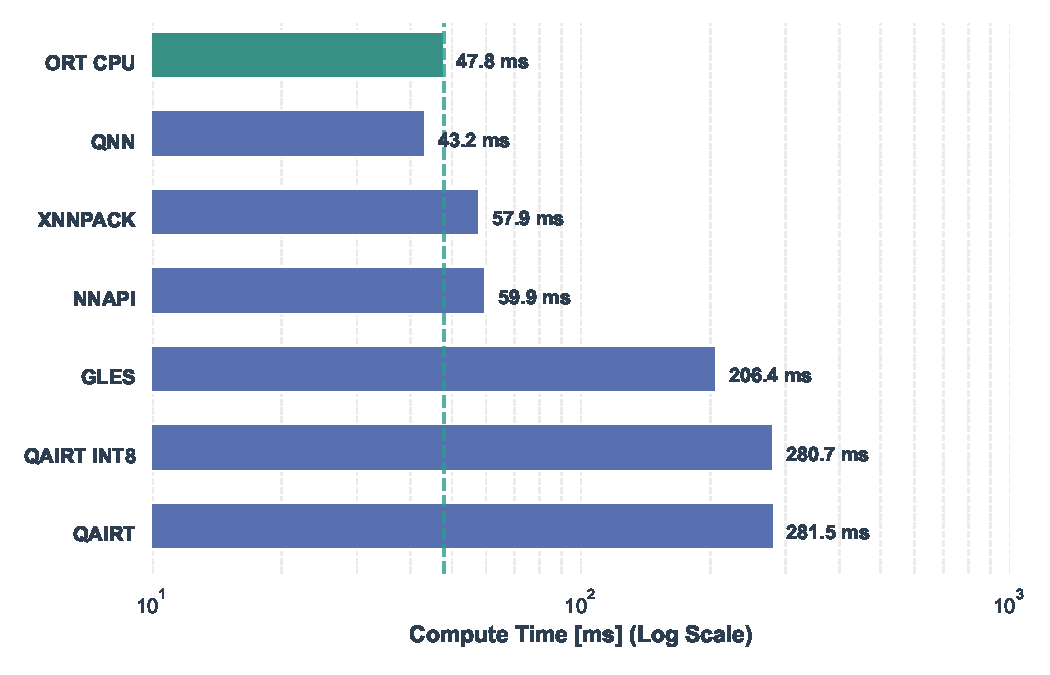
\includegraphics[width=0.95\textwidth]{figures/globalna_primerjava_casov.pdf}
\caption{Globalni primerjalni prikaz povprečnih časov izvajanja particije \texttt{block\_0\_node} MLP za vse uspešne izvajalne poti.}
\label{fig:global_chart}
\end{figure}

Ugotovitve po analizi zbranih podatkov lahko razdelimo na tri glavna nizkonivojska ozka grla, ki mobilnim strojno pospešenim okoljem preprečujejo doseganje višjih hitrosti pri fizikalnih simulacijah oblačil z nevronskimi mre\-ža\-mi nad grafi:

\begin{itemize}
\item \textbf{Dinamična narava grafnih struktur:} Modeli, kot je HOOD, v vsakem časovnem koraku dinamično spreminjajo dimenzije matrik zaradi uveljavljanja aktivne maske telesa in iskanja sosedov. Mobilni pospeševalniki znotraj knjižnice Qualcomm QAIRT ali vmesnika NNAPI pa zahtevajo vnaprej fiksirane pomnilniške alokacije (angl.\ \textit{static tensor shapes}). Dinamično spreminjanje dimenzij med tekom simulacije zahteva dodatne alokacije oziroma prilagoditve poti izvajanja, kar upočasni izvajanje.
\item \textbf{Učinkovitost računanja na mobilnih enotah GPE:} Neposredna primerjava na isti particiji je jasno pokazala, da optimizirana domorodna koda v jeziku C++ za senčilnike GLES ($206{,}43\text{ ms}$) ter neposredne poti QAIRT ($281{,}51\text{ ms}$) niso uspele prehiteti osnovne poti na CPE. Glavna težava je sam čas izvajanja gostih struktur MLP na mobilni grafični enoti. Mobilni strojni gonilniki teh specifičnih oblik plasti s plavajočo vejico ne uspejo vzporedno zaposliti v zadostni meri, da bi prehiteli izjemno močna in optimizirana procesorska jedra in hkrati pokrili stroške prenosa podatkov na GPE.
\item \textbf{Nezdružljivost naprednih matematičnih operacij:} Ker mobilna namenska okolja neposredno ne podpirajo operacij, kot sta plastna normalizacija \texttt{LayerNorm} ali specifična agregacija \texttt{scatter\_sum}, se mora računski tok v nekaterih testiranih mobilnih poteh nenehno vračati na procesor CPE. To preklapljanje konteksta in deljenje grafov povzročata dodatne časovne kazni.
\end{itemize}

Iz teh ugotovitev izhajajo jasni zaključki o prenosu tovrstnih fizikalnih grafnih nevronskih mrež na mobilne naprave. Čeprav klasičen, dobro optimiziran procesorski cevovod ponuja najvišjo stabilnost in hitrost med vsemi testiranimi mobilnimi potmi, so ti časi še vedno bistveno prepočasni za realnočasovno simulacijo. Najboljši doseženi skupni čas okvirja na najnovejši napravi Samsung Galaxy S26+ znaša 2,66 s, na referenčni napravi OnePlus pa kar 15,9 s. To pomeni, da se mobilna izvedba trenutno ne približa povprečnemu času izvajanja modela HOOD na namiznem računalniku, ki znaša 150 ms za en časovni okvir. Za testirane oblike in velikosti perceptronov MLP mobilna enota GPE ne premaga procesorja CPE, saj strojni pospeševalniki pri teh srednje velikih MLP-jih ne ponujajo nikakršnih hitrostnih prednosti. Morebiten prehod na izvajanje na enoti GPE bi zahteval korenito transformacijo celotne mreže v fiksne dimenzije z uveljavitvijo praznih dopolnitev ter zamenjavo plasti normalizacije.



%----------------------------------------------------------------
% Poglavje (Chapter) 7
%----------------------------------------------------------------
\chapter{Zaključek in nadaljnje delo}
\label{ch:zaključek_in_nadaljnje_delo}

V magistrskem delu smo obravnavali problem realnočasovne simulacije tkanine na mobilnih napravah. Cilj naloge je bil preveriti, ali je mogoče sodobne nevronske modele za simulacijo tkanin, ki so bili prvotno razviti za namizna okolja, učinkovito prenesti na mobilno strojno opremo. Pri tem smo se osredotočili na dva vidika: na primerjavo obstoječih modelov simulacije tkanin ter na praktično mobilno implementacijo izbranega modela HOOD.

V prvem delu naloge smo izvedli primerjalno analizo modelov TailorNet, HOOD in ContourCraft na enotni eksperimentalni postavitvi. Za referenčno simulacijo smo uporabili nCloth v okolju Maya, vhodne podatke pa smo standardizirali z uporabo gibanj iz arhiva AMASS in parametričnega modela telesa SMPL. Rezultati so pokazali, da sta modela HOOD in ContourCraft geometrijsko in fizikalno bistveno natančnejša od modela TailorNet, pri čemer je HOOD dosegel tudi najboljše razmerje med natančnostjo in časovno učinkovitostjo. Na podlagi teh rezultatov smo HOOD izbrali kot najprimernejšega kandidata za mobilno implementacijo.

V drugem delu naloge smo razvili mobilni inferenčni cevovod za Android in ga postopoma ovrednotili na več izvajalnih poteh. Ker neposreden izvoz celotnega modela HOOD v enoten graf ONNX ni bil izvedljiv, smo model razdelili na manjše particije, dinamično grafno logiko pa ponovno implementirali neposredno v mobilni aplikaciji. Kot referenčno osnovo smo vzpostavili popolnoma delujočo pot z ogrodjem ONNX Runtime na procesorju CPE. Ta osnova je ohranila popolno numerično natančnost, vendar je bila časovno zelo zahtevna: na napravi OnePlus Nord CE 3 Lite je povprečni čas obdelave enega časovnega okvira znašal $15{,}85$ s, na zmogljivejši napravi Samsung Galaxy S26+ pa $2{,}66$ s.

Nato smo preizkusili več različnih strategij strojnega pospeševanja: ponudnika izvajanja NNAPI in XNNPACK, prilagojeno različico ORT s ponudnikom QNN, lastne prototipe z računskimi senčilniki GLES, zunanji izvajalnik QNN, ogrodje LiteRT ter neposredno domorodno integracijo knjižnice Qualcomm QAIRT. Ključna ugotovitev vseh teh poskusov je bila, da nobena od testiranih mobilnih poti ni presegla optimizirane osnove ORT CPE na isti particiji \texttt{block\_0\_node} MLP.

Pri standardnih ponudnikih izvajanja sta NNAPI in XNNPACK sicer uspešno izvedla izolirano particijo, vendar sta bila oba počasnejša od osnovnega procesorja. Pri prilagojeni poti ORT s ponudnikom QNN je profiliranje pokazalo, da nobena operacija ni bila dejansko odložena na pospeševalnik, zato je bil navidezni časovni dobiček posledica drugačnega načrta izvajanja na CPE in ne resničnega strojnega pospeševanja. Poskusi s kvantizacijo v okviru ORT prav tako niso prinesli dejanske koristi in so povzročili degradacijo numerične natančnosti.

Podobno negativni so bili tudi rezultati pri uporabi senčilnikov GLES. Kotlin upravljana izvedba kodirnika vozlišč je bila bistveno počasnejša od procesorske osnove, zato smo razvili še domorodno C++ različico za particijo \texttt{block\_0\_node} MLP. Tudi po optimizacijah, odpravi dodatnih kopiranj pomnilnika in prilagoditvi senčilnika je ta pot ostala približno $4{,}3$-krat počasnejša od ORT CPE. Podrobnejša instrumentacija je pokazala, da glavni strošek ni bil prenos podatkov, temveč čakanje na dokončanje računanja na grafični enoti, kar pomeni, da je bila glavna omejitev neučinkovitost lastne implementacije gostega perceptrona MLP na mobilni GPE.

Zunanji izvajalnik QNN je pokazal, da je mogoče doseči funkcionalno pravilne rezultate tudi zunaj aplikacijskega procesa, vendar so stroški prenosa podatkov, orkestracije in datotečnega vhoda to pot naredili prepočasno in nezanesljivo. Ogrodje LiteRT je pri izpeljanih podmodelih HOOD povzročilo numerični odmik, kar je za fizikalno simulacijo nesprejemljivo. Tudi neposredna integracija knjižnice Qualcomm QAIRT na GPE ni prinesla pričakovane prednosti: pri izolirani particiji \texttt{block\_0\_node} MLP je bila pot QAIRT približno $5{,}9$-krat počasnejša od ORT CPE, kvantizacija pa ni izboljšala časa izvajanja in je hkrati opazno poslabšala natančnost.

Glavni prispevek naloge je, da smo vzpostavili enoten primerjalni cevovod za več modelov simulacije tkanin in za mobilno ovrednotenje izbranega modela HOOD. Eksperimentalni rezultati so pokazali dva ključna problema pri prenosu modela na mobilne naprave. Prvi problem je slabo ujemanje med dinamično heterogeno grafno strukturo modela HOOD in mobilnimi izvajalnimi ogrodji, zaradi česar celotnega cevovoda ni bilo mogoče učinkovito prenesti kot enoten statični graf. Drugi problem pa je, da tudi pri izoliranih statičnih MLP-particijah testirane poti na GPE niso prehitele dobro optimizirane procesorske izvedbe ORT CPE.

Končni zaključek naloge je, da mobilna izvedba modela HOOD v obravnavani obliki trenutno še ni primerna za realnočasovno simulacijo tkanine. Kljub temu delo jasno pokaže, kje so ključne omejitve in kateri deli arhitekture bi zahtevali korenitejšo prilagoditev za uspešen prehod na mobilne naprave.

\subsubsection{Nadaljnje delo}
Rezultati naloge odpirajo več smiselnih smeri za nadaljnje delo.

Najbolj neposredna možnost je arhitekturna prilagoditev modela HOOD za mobilna izvajalna okolja. Trenutna zasnova temelji na dinamični gradnji grafov, aktivni maski telesa in spremenljivih dimenzijah tenzorjev, kar je slabo združljivo z mobilnimi pospeševalniki. Smiselno bi bilo raziskati preoblikovanje modela v bolj statično obliko z uporabo praznih dopolnitev, fiksnih dimenzij in vnaprej pripravljenih povezav, s čimer bi bil model primernejši za izvajanje na GPE.

Pomembna smer nadaljnjega dela je tudi globlja optimizacija posameznih particij. V nalogi smo pokazali, da srednje veliki perceptroni MLP na mobilni enoti GPE niso nujno hitrejši od procesorja CPE. Nadaljnje raziskave bi zato lahko vključevale razvoj bolj specializiranih senčilnikov, agresivnejše zlivanje operacij ali uporabo alternativnih nizkonivojskih API-jev, ki bi bolje izkoristili strojno opremo kot prototipna izvedba z GLES.

Dolgoročno bi bilo smiselno razmisliti tudi o spremembi samega modela simulacije. Model HOOD je bil izbran zaradi visoke kakovosti simulacije, vendar ni bil zasnovan z mislijo na mobilna okolja. Nadaljnje raziskave bi zato lahko vodile v razvoj nove arhitekture, ki bi imela drugačne velikosti particij MLP, manj tipov relacij, manj dinamičnih odločitev med izvajanjem ter neposredno prilagojenost operacijam, ki jih mobilni pospeševalniki učinkovito podpirajo.

Na podlagi opravljenega dela lahko sklenemo, da področje mobilne simulacije tkanin ostaja odprt raziskovalni problem. Ključ do uporabne realnočasovne rešitve verjetno ne bo v neposrednem prenosu obstoječih namiznih modelov na mobilne naprave, temveč v sočasni prilagoditvi modela, podatkovne predstavitve in izvajalnega okolja specifičnim omejitvam mobilne strojne opreme.



%----------------------------------------------------------------
% SLO: bibliografija
% ENG: bibliography
%----------------------------------------------------------------
\bibliographystyle{elsarticle-num}

%----------------------------------------------------------------
% SLO: odkomentiraj za uporabo zunanje datoteke .bib (ne pozabi je potem prevesti!)
% ENG: uncomment to use .bib file (don't forget to compile it!)
%----------------------------------------------------------------
\bibliography{bibliography}
\end{document}
